% ==============================================================================
% Carlos Subiabre Saldivia - Ingeniería Civil Informática - U. Aysén
% ==============================================================================

\documentclass[12pt, letterpaper, oneside]{memoir}

% --- Codificación y Lenguaje ---
\usepackage[utf8]{inputenc}
\usepackage[T1]{fontenc}
\usepackage[spanish,es-noshorthands]{babel}
\usepackage{csquotes}
% --- Tipografía Profesional ---
\usepackage{lmodern} 
\usepackage{mathpazo} 
\linespread{1.3}

% --- Paquetes Esenciales y de Ingeniería ---
\usepackage{graphicx}
\usepackage{amsmath, amssymb}
\usepackage{booktabs}
\usepackage{multirow}
\usepackage{siunitx}
\usepackage{numprint}
\npthousandsep{.}
\npdecimalsign{,}
\sisetup{
  output-decimal-marker = {,},
  group-separator = {.},
  group-minimum-digits = 4,
  per-mode = symbol,
  detect-all = true,
  parse-numbers = false
}

% --- Paquetes para Diagramas (TikZ) ---
\usepackage{tikz}
\usetikzlibrary{arrows.meta, chains, positioning, shapes.geometric}

% --- Configuración de Bibliografía (biblatex) ---
% --- Configuración de Bibliografía (biblatex) ---
\usepackage[backend=biber, style=apa, sorting=nyt]{biblatex}
\addbibresource{bibliografia.bib} % Nombre de tu archivo .bib

% --- Configuración de Hipervínculos y Referencias Inteligentes ---
\usepackage[hidelinks]{hyperref}
\usepackage[spanish,nameinlink]{cleveref}

% --- Configuración para Listados de Código ---
\usepackage{listings}
\usepackage{xcolor}
\definecolor{codegreen}{rgb}{0,0.6,0}
\definecolor{codegray}{rgb}{0.5,0.5,0.5}
\definecolor{codepurple}{rgb}{0.58,0,0.82}
\definecolor{backcolour}{rgb}{0.97,0.97,0.95}
\lstdefinestyle{pythonstyle}{
    backgroundcolor=\color{backcolour}, commentstyle=\color{codegreen},
    keywordstyle=\color{magenta}, numberstyle=\tiny\color{codegray},
    stringstyle=\color{codepurple}, basicstyle=\footnotesize\ttfamily,
    breakatwhitespace=false, breaklines=true, captionpos=b, keepspaces=true,
    numbers=left, numbersep=5pt, showspaces=false, showstringspaces=false,
    showtabs=false, tabsize=2, language=Python
}
\lstset{style=pythonstyle}

% ==============================================================================
% DISEÑO DEL DOCUMENTO (Controlado por memoir)
% ==============================================================================
\chapterstyle{veelo}
\setstocksize{11in}{8.5in}
\settrimmedsize{\stockheight}{\stockwidth}{*}
\setlrmarginsandblock{3cm}{2.5cm}{*}
\setulmarginsandblock{2.5cm}{2.5cm}{*}
\setheadfoot{16pt}{12pt}
\checkandfixthelayout
\makepagestyle{main}
\makeevenhead{main}{\thepage}{}{\leftmark}
\makeoddhead{main}{\rightmark}{}{\thepage}
\makepagestyle{plain}
\makeevenhead{plain}{\thepage}{}{}
\makeoddhead{plain}{}{}{\thepage}
\pagestyle{main}
\aliaspagestyle{chapter}{plain}
\firmlists
\renewcommand{\listtablename}{Índice de Cuadros}
% ==============================================================================
% INICIO DEL DOCUMENTO
% ==============================================================================
\begin{document}

\frontmatter
\begin{titlingpage}
    \centering % Centra todo el contenido horizontalmente
    
    \vfill 
    
    \includegraphics[width=0.25\textwidth]{logo_uaysen.png}
    \vspace{1.5cm}
    
    {\Large \scshape Universidad de Aysén}\\[0.5cm]
    {\large \scshape Departamento de Ciencias Naturales y Tecnología}\\[0.5cm]
    {\large \scshape Carrera de Ingeniería Civil Informática}
    
    \vfill
    
    \rule{\textwidth}{1pt}\vspace*{0.4cm}
    % --- TÍTULO AJUSTADO ---
    {\LARGE \bfseries Diseño de un Modelo de Simulación \\ 
    para el Análisis de Resiliencia en la \\ 
    Cadena de Suministro de Gas Licuado de Petróleo  de Aysén}\\[0.4cm]
    \rule{\textwidth}{1pt}
    
    \vspace{1cm}
    {\large Memoria para optar al título de Ingeniero Civil Informático}
    
    \vfill
    
    \begin{large}
    \begin{tabular}{ll}
        \textbf{Autor:} & Carlos Subiabre Saldivia \\
        \textbf{Mentora:} & Natacha Pino Acuña \\
    \end{tabular}
    \end{large}
    
    \vspace{2cm}
    
    {\large Coyhaique, Chile}\\[0.5cm]
    {\large 2025}
    
    \vfill
    
\end{titlingpage}
% --- Agradecimientos ---
\chapter*{Agradecimientos}
\addcontentsline{toc}{chapter}{Agradecimientos} % Añadir a la tabla de contenidos

Deseo expresar mi agradecimiento a las personas que hicieron posible la 
realización de esta memoria.

A mi familia, por su constante apoyo y paciencia a lo largo de mis años de 
estudio. Su confianza fue fundamental para llegar a esta etapa.

A mi mejor amiga, por su invaluable amistad y por su 
aliento en los momentos más difíciles de este proceso.

A mi mentora, Profesora Natacha Pino Acuña, por su guía, tiempo y 
dedicación. Sus conocimientos y consejos fueron esenciales para el 
desarrollo de esta memoria.

\clearpage

% --- Resumen ---
\chapter*{Resumen}
\addcontentsline{toc}{chapter}{Resumen}

La cadena de suministro de Gas Licuado de Petróleo (GLP) en la Región de Aysén 
constituye un sistema sociotécnico de alta criticidad, caracterizado por una 
topología logística sin redundancia y una capacidad de respuesta endógena 
insuficiente para mitigar las disrupciones exógenas recurrentes. El 
diagnóstico técnico actual, si bien es exhaustivo, es de naturaleza estática 
y carece de herramientas para evaluar dinámicamente el impacto de los riesgos 
o el retorno en resiliencia de las inversiones propuestas.

Este trabajo de titulación aborda dicha brecha metodológica mediante el 
diseño, implementación y validación de un prototipo de simulación de eventos 
discretos. El artefacto computacional desarrollado modela la interacción de 
los parámetros logísticos clave ---capacidad de almacenamiento, políticas de 
inventario, demanda estocástica y, crucialmente, la frecuencia y duración de 
las interrupciones de la ruta de suministro--- concentrados en el nodo de 
almacenamiento primario de Coyhaique, que actúa como centro neurálgico del 
sistema regional.

El objetivo es crear un laboratorio virtual que permita cuantificar la 
resiliencia del sistema bajo diferentes escenarios. Mediante un diseño de 
experimentos formal, se evaluará la sensibilidad del sistema a distintos 
parámetros, buscando confirmar la hipótesis de que la resiliencia es 
significativamente más sensible a la duración de las disrupciones de ruta 
que a las variaciones en la capacidad de almacenamiento. El prototipo 
validado sienta una base metodológica para la toma de decisiones informadas, 
instrumentalizando una recomendación explícita de la política pública 
regional y contribuyendo al fortalecimiento de la seguridad energética de 
Aysén.

\vspace{1cm}
\noindent\textbf{Palabras Clave:} Simulación de Eventos Discretos, 
Resiliencia de Cadenas de Suministro, Gestión de Inventarios, Análisis de 
Riesgos, Seguridad Energética, Ingeniería de Sistemas.
\tableofcontents
\clearpage
\listoffigures
\clearpage
\listoftables



\mainmatter
\chapter{Introducción}
\label{chap:introduccion}

\section{Contexto General}

La gestión de cadenas de suministro en zonas geográficamente aisladas representa un desafío de ingeniería que excede las soluciones logísticas convencionales. A diferencia de los sistemas conectados a redes troncales robustas, donde la variabilidad se amortigua mediante redundancias múltiples, las zonas aisladas operan bajo condiciones de fragilidad estructural. En estos entornos, la continuidad del servicio no depende únicamente de la capacidad de almacenamiento estático, sino de la dinámica temporal de reabastecimiento frente a interrupciones estocásticas.

La literatura en ingeniería de sistemas define la resiliencia no como la ausencia de fallas, sino como la capacidad de un sistema para absorber perturbaciones y recuperar su estado operativo. Sin embargo, en el contexto energético, las herramientas tradicionales de planificación suelen basarse en modelos deterministas —promedios anuales y márgenes de seguridad estáticos— que fallan al capturar la complejidad de eventos de "cola pesada", como disrupciones climáticas extremas o cortes de ruta prolongados.

\section{Contexto Regional}

La Región de Aysén presenta un caso paradigmático de aislamiento energético extremo. Sin conexión terrestre continua con el resto de Chile y dependiente de rutas marítimas y carreteras vulnerables a factores climáticos, la región importa el 100% de sus combustibles fósiles. El Gas Licuado de Petróleo (GLP) no es aquí un combustible suntuario, sino un insumo crítico de subsistencia, utilizado masivamente para calefacción residencial en un clima donde las temperaturas invernales descienden frecuentemente bajo cero.

El sistema opera bajo un oligopolio de distribución conformado por tres actores principales: \textbf{Abastible, Lipigas y Gasco}. Estas empresas concentran su inventario en un único nodo logístico central en Coyhaique, con una capacidad de almacenamiento combinada de \textbf{431 toneladas métricas (TM)}. Esta infraestructura debe abastecer una demanda regional que exhibe una fuerte estacionalidad, alcanzando picos en invierno que ponen a prueba la capacidad del sistema.

La cadena logística implica un transporte multimodal complejo: desembarque marítimo en puertos intermedios (Puerto Chacabuco o Puerto Cisnes) y transporte terrestre vía Ruta 7. Esta configuración crea un sistema con un "punto único de falla" (Single Point of Failure): si el inventario en el nodo central se agota debido a un bloqueo en la ruta de suministro, no existen sustitutos inmediatos viables, desencadenando una crisis de seguridad energética regional.

\section{Problemática}

El problema central no es la falta de combustible en el mercado global, sino la incapacidad del sistema logístico regional para garantizar la disponibilidad continua frente a la variabilidad conjunta de la demanda y el suministro.

Los datos técnicos, corroborados por el informe \cite{CNE2024}, revelan una brecha estructural alarmante: la capacidad instalada de 431 TM proporciona una autonomía teórica de apenas \textbf{8,2 días} bajo condiciones de demanda invernal. Sin embargo, la historia de disrupciones de la Ruta 7 muestra eventos de bloqueo —causados por nevadas, derrumbes o conflictos gremiales— que pueden extenderse hasta por \textbf{21 días}, como se evidenció durante las protestas en Argentina en 2021.

Esta disparidad (8,2 días de autonomía vs. 21 días de riesgo de corte) define la vulnerabilidad del sistema. Actualmente, la planificación se realiza mediante herramientas estáticas que ignoran esta estocasticidad, resultando en un sistema reactivo donde las medidas de mitigación se activan solo cuando la crisis es inminente.

\section{Brecha Detectada}

Existe una desconexión fundamental entre la complejidad del problema físico (un sistema dinámico, estocástico y no lineal) y las herramientas utilizadas para resolverlo (modelos estáticos lineales).

Mientras que la ingeniería industrial moderna utiliza ampliamente la Simulación de Eventos Discretos (DES) para optimizar líneas de producción y logística portuaria, su aplicación en la planificación de seguridad energética regional en Chile es incipiente. No existe actualmente un modelo computacional validado que permita a los tomadores de decisiones en Aysén responder preguntas del tipo: "¿Cuál es la probabilidad de desabastecimiento si la demanda crece un 10% y ocurre un bloqueo de ruta de 7 días en julio?". La falta de esta herramienta obliga a tomar decisiones de inversión basándose en intuición, aumentando el riesgo de falla de servicio.

\section{Requerimientos de la Solución}

Para cerrar esta brecha, se requiere una solución desde la ingeniería informática que permita modelar la complejidad temporal del sistema. No basta con una ecuación cerrada; se necesita un artefacto de software capaz de simular el comportamiento del sistema a través del tiempo.

La solución debe satisfacer los siguientes requerimientos técnicos para ser efectiva:
1.  **Capacidad de Simulación Estocástica:** El software debe implementar algoritmos de generación de números pseudoaleatorios para modelar la incertidumbre en la demanda (ruido gaussiano) y en las disrupciones de ruta (procesos de llegada de Poisson).
2.  **Granularidad Temporal:** El modelo debe operar con un reloj de simulación discreto capaz de evaluar el estado del sistema día a día, capturando la acumulación y agotamiento de inventarios de forma dinámica.
3.  **Parametrización Flexible:** Debe permitir configurar distintos escenarios (aumento de capacidad de tanques a 681 TM, cambios en la flota, variación de políticas de stock) sin reescribir el código fuente.
4.  **Reproducibilidad:** A diferencia de los análisis ad-hoc, la solución debe ser un software ejecutable que permita correr experimentos de Monte Carlo (miles de iteraciones) para obtener resultados estadísticamente significativos.

En resumen, se propone el desarrollo de un simulador de eventos discretos ("Digital Twin" simplificado) que transforme la incertidumbre inherente del entorno en métricas de riesgo cuantificables.

\chapter{Planteamiento del Problema}
\label{chap:planteamiento-problema}

La Región de Aysén enfrenta un riesgo sistémico en su suministro de GLP. Este capítulo caracteriza el sistema (demanda, infraestructura, actores), identifica sus vulnerabilidades (exógenas y endógenas), y argumenta por qué los métodos de análisis actuales (matrices de riesgo estáticas) son insuficientes para evaluar la resiliencia dinámica del sistema.

\section{Caracterización del Sistema}
\label{sec:caracterizacion-sistema}

El sistema de suministro de GLP en Aysén opera bajo condiciones que lo
definen como un sistema complejo y crítico. Su criticidad se deriva de la
confluencia de una demanda energética elevada, una estructura de mercado
oligopólica y una infraestructura precaria.

\subsection{Demanda energética y crecimiento proyectado}

La demanda energética de la región es un factor distintivo a nivel nacional. 
Con un consumo per cápita de \SI{27.25}{Gcal}, que excede en un 65\% la 
media de Chile, la población depende intensivamente de un flujo energético 
constante para sostener funciones básicas. El GLP satisface nichos de 
consumo ---cocción de alimentos y agua caliente sanitaria--- para los cuales 
no existen sustitutos inmediatos a gran escala. Esta inelasticidad 
fundamental de la demanda convierte al GLP en un recurso de alta prioridad 
social, cuya interrupción tiene consecuencias directas e inmediatas sobre 
el bienestar de la población.

Adicionalmente, la demanda no es estática. El sistema enfrenta un 
crecimiento sostenido del \SI{3.8}{\percent} anual, impulsado por el 
desarrollo demográfico y económico de la región. A esto se suma un factor 
disruptivo futuro: la proyectada incorporación de una central térmica que 
consumirá \SI{14.4}{ton/día} de GLP. Este crecimiento y cambio estructural 
implican que la presión sobre la ya frágil cadena de suministro se 
intensificará de manera no lineal en los próximos años.

\subsection{Estructura de la cadena de suministro}

% --- SECCIÓN PROFUNDIZADA CON ANÁLISIS DE LA RUTA ---
La estructura de la cadena de suministro, detallada en el informe de 
referencia~\cite{CIEP2025}\footnote{El informe, encargado por la Seremía de 
Energía de Aysén, fue finalizado y presentado en 2025. A la fecha de esta 
publicación, se encuentra en proceso de difusión pública.}, se caracteriza
por una topología logística 
lineal con una dependencia absoluta de fuentes exógenas. El informe es 
categórico al afirmar que ``La totalidad del gas licuado que llega a la 
región, lo hace vía camiones que transitan por el paso Huemules desde 
Argentina''. Este diseño, carente de redundancia, convierte a la ruta 
terrestre en un punto único de falla (\textit{Single Point of Failure}) de 
manual. La magnitud de esta dependencia se cuantifica en el hecho de que el 
86\% del recorrido terrestre desde la planta de Cabo Negro hasta Coyhaique 
transcurre por territorio argentino, lo que implica que la soberanía 
logística y la seguridad del suministro regional están estructuralmente 
comprometidas por la dinámica de un país vecino.

\section{Análisis de vulnerabilidades}
\label{sec:analisis-vulnerabilidades}

El sistema presenta vulnerabilidades tanto exógenas (amenazas externas) como endógenas (limitaciones de capacidad interna).

\subsection{Vulnerabilidades exógenas}

% --- SECCIÓN PROFUNDIZADA CON CUANTIFICACIÓN DEL RIESGO ---
El principal vector de riesgo es la incertidumbre estocástica en el 
aprovisionamiento. El informe de riesgos~\cite{CIEP2025} identifica dos 
amenazas dominantes. Primero, el evento de ``Nevadas / Cierre cruce 
fronterizo'' (Tag \#57), clasificado con una probabilidad de Nivel 4 (``Casi 
Seguro''), lo que implica una frecuencia de ocurrencia de ``al menos una vez 
cada tres meses''. Segundo, el riesgo de ``Conflicto social en Argentina'' 
(Tag \#45), que, aunque menos frecuente, ha demostrado la capacidad de 
paralizar el suministro por períodos de hasta tres semanas. Esta 
realidad es corroborada por la autoridad energética regional, quien 
identifica la ``conflictividad social'' y la ``mantención de los caminos'' 
en Argentina como la principal amenaza para la continuidad del suministro 
(Laibe, T., comunicación personal, 11 de junio, 2025). El sistema, por tanto, 
enfrenta amenazas recurrentes y de duración prolongada que introducen una 
alta variabilidad en el tiempo de entrega (\textit{lead time}).

\subsection{Vulnerabilidades endógenas}

La capacidad de almacenamiento en Coyhaique es de 431 TM (Abastible 150, Lipigas 240, Gasco 41)~\cite{CIEP2025}, proporcionando 8,2 días de autonomía vs. disrupciones documentadas de hasta 21 días.

El informe CIEP 2025 identifica que "Gasco tiene una capacidad demasiado reducida para su nivel de ventas" (41 TM = 0,78 días de autonomía). Esta situación refleja un Dilema del Prisionero en el mercado oligopólico: minimizar costos de inventario individualmente (estrategia racional) degrada la resiliencia colectiva.

\textbf{Propuesta 10.4 (Gasco):} El informe documenta que Gasco está desarrollando un proyecto de expansión para incrementar su capacidad en 250 TM (de 41 a 291 TM), elevando la capacidad total del sistema de 431 TM a 681 TM. La inversión estimada es \$1,5 millones USD. Esta expansión aumentaría la autonomía teórica del sistema de 8,2 a 13 días.

El presente trabajo evalúa cuantitativamente el retorno en resiliencia de esta inversión bajo diferentes escenarios de disrupciones.

\section{Limitaciones del diagnóstico actual}
\label{sec:insuficiencia-marcos}

\subsection{Vacío en la planificación energética regional}

La 'Política Energética 2050 Región de Aysén' se enfoca exclusivamente en el sector eléctrico, omitiendo la cadena de suministro de combustibles.

\subsection{Análisis estático vs. dinámico}

El informe CIEP 2025 es exhaustivo pero estático: identifica riesgos mediante una matriz de probabilidad × impacto, pero no puede cuantificar:

\begin{itemize}
    \item ¿Cuánto tiempo puede operar el sistema bajo disrupciones largas?
    \item ¿Qué tan frecuentemente fallará el sistema (quiebres de stock)?
    \item ¿Cuál es el retorno en resiliencia de la inversión de \$1,5M USD (Propuesta 10.4)?
\end{itemize}

\subsection{Gestión reactiva de crisis}

La gestión operativa de crisis se basa en protocolos manuales: "llamar a todas las empresas, construir un Excel y sacar una foto de cuánta disponibilidad de combustible hay" (Laibe, T., comunicación personal, 11 de junio, 2025). No existe una herramienta de análisis dinámico.

\subsection{Pregunta que el diagnóstico actual no puede responder}

\textit{¿Cuál es la reducción en probabilidad de quiebre de stock que genera la inversión de \$1,5M USD (Propuesta 10.4 de Gasco), bajo un escenario de disrupciones con frecuencia 4 eventos/año y duración estocástica de hasta 21 días?}

Esta tesis desarrolla el modelo para responder esta pregunta.
\chapter{Hipótesis y Pregunta de Investigación}
\label{chap:hipotesis}

El análisis del problema, expuesto en el \cref{chap:planteamiento-problema}, 
revela un sistema sociotécnico complejo, dominado por la interacción de 
variables estocásticas y decisiones estratégicas. La disonancia entre la 
magnitud de las amenazas exógenas y la limitada capacidad de respuesta 
endógena sugiere que no todos los parámetros del sistema contribuyen de 
igual manera a su vulnerabilidad global. Para abordar esta complejidad de 
manera científica, es imperativo formular una pregunta de investigación que 
guíe el diseño de una herramienta de análisis cuantitativo, y una hipótesis 
falsificable que postule una relación de sensibilidad entre los factores 
críticos del sistema.

\section{Pregunta de Investigación}
\label{sec:pregunta-investigacion}

Considerando la caracterización del sistema, sus vulnerabilidades y la
brecha metodológica identificada en los marcos de análisis actuales, la
pregunta central que esta investigación busca responder es:
\begin{quote}
    \textit{¿Cómo diseñar, implementar y validar un modelo de simulación de
    eventos discretos para cuantificar el impacto de parámetros logísticos
    críticos ---tales como la duración de las disrupciones de ruta y las
    políticas de inventario--- sobre la resiliencia del sistema de suministro
    de GLP en Aysén?}
\end{quote}
Esta pregunta aborda tanto la construcción del modelo como la validación de
su utilidad para analizar este sistema sociotécnico.

\section{Hipótesis Central}
\label{sec:hipotesis}

Como una respuesta conjetural y testable a la pregunta de investigación, y 
derivada directamente de la disonancia identificada en el planteamiento del 
problema, se postula la siguiente hipótesis central:
\begin{quote}
    \textbf{Hipótesis:} La resiliencia del sistema de suministro de GLP de 
    Aysén, cuantificada a través de métricas de rendimiento como el Nivel de 
    Servicio, exhibe una sensibilidad significativamente mayor a la 
    variabilidad de los parámetros exógenos que a la de los parámetros 
    endógenos. Específicamente, se postula que la elasticidad de la 
    resiliencia con respecto a la duración de las disrupciones de ruta 
    es superior a su elasticidad con respecto a las variaciones en la 
    capacidad de almacenamiento primario.
\end{quote}
Esta hipótesis formaliza la intuición de que la magnitud de las amenazas 
externas (ej. un corte de 21 días) es el factor dominante que gobierna el 
comportamiento del sistema, por sobre las mejoras incrementales en la 
capacidad de respuesta interna (ej. aumentar el inventario de 8 a 12 días 
de autonomía). El diseño experimental, detallado en el 
\cref{chap:metodologia}, está específicamente concebido para proveer la 
evidencia estadística necesaria para confirmar o refutar esta afirmación, 
jerarquizando así las palancas de acción más efectivas para fortalecer la 
seguridad energética regional.
% --- SIN CAMBIOS, YA ES CORRECTO ---
\chapter{Objetivos}
\label{chap:objetivos}

Para abordar la brecha metodológica identificada en el \cref{chap:planteamiento-problema} 
y responder a la pregunta de investigación formulada, el presente proyecto se 
estructura en torno a un conjunto de objetivos jerárquicos. Estos objetivos 
guían el proceso de diseño, desarrollo y validación del artefacto 
computacional propuesto, asegurando un enfoque sistemático para la creación 
de un laboratorio virtual que permita el análisis dinámico de la resiliencia 
del sistema de suministro de GLP.

\section{Objetivo General}
\label{sec:objetivo-general}

Diseñar un prototipo de simulación de eventos discretos, validado 
computacionalmente, para cuantificar el impacto de parámetros logísticos 
críticos sobre la resiliencia del sistema de suministro de GLP en el nodo 
Coyhaique.

\section{Objetivos Específicos}
\label{sec:objetivos-especificos}

La consecución del objetivo general se desglosa en tres fases metodológicas 
secuenciales, cada una representada por un objetivo específico que define 
una etapa clave del proceso de investigación y desarrollo:

\begin{enumerate}
    \item \textbf{Modelar} la dinámica conceptual de la cadena de suministro 
    de GLP en Coyhaique, realizando una abstracción formal de sus 
    componentes, procesos y parámetros clave a partir de la información 
    técnica disponible.
    
    \item \textbf{Implementar} un prototipo computacional del modelo de 
    simulación, desarrollando una arquitectura de software parametrizable 
    que traduzca el modelo conceptual a un artefacto funcional y 
    experimental.
    
    \item \textbf{Evaluar} la resiliencia del sistema mediante la ejecución 
    de un diseño experimental sobre el prototipo validado, utilizando la 
    simulación para generar la evidencia empírica necesaria para confirmar 
    o refutar la hipótesis de trabajo.
\end{enumerate}
\chapter{Marco Conceptual y Matemático}
\label{chap:marco-teorico}

La construcción de un simulador para sistemas logísticos complejos no es un ejercicio trivial de programación, sino una aplicación sistemática de principios de la teoría de la computación, la estadística matemática y la investigación de operaciones. Este capítulo establece los fundamentos formales que validan la arquitectura del software, detallando los algoritmos específicos seleccionados para la gestión del tiempo discreto, la generación de entropía artificial y la modelación de procesos estocásticos.

\section{Teoría de Simulación de Eventos Discretos (DES)}
La Simulación de Eventos Discretos se distingue fundamentalmente de la simulación continua por su tratamiento del tiempo y del estado del sistema.

\subsection{Definición Formal del Sistema}
Según \textcite{Banks2010}, un sistema de eventos discretos se modela mediante una tupla de variables de estado $S(t)$ cuya trayectoria es constante a tramos (\textit{piecewise constant}). Matemáticamente, si definimos una secuencia de eventos $e_1, e_2, \dots, e_n$ que ocurren en los tiempos $t_1 < t_2 < \dots < t_n$, el estado del sistema permanece inmutable en el intervalo $[t_i, t_{i+1})$. Esta propiedad es la que permite al algoritmo de simulación ``saltar'' en el tiempo, avanzando el reloj global (CLOCK) directamente de $t_i$ a $t_{i+1}$ sin incurrir en el costo computacional de integrar los pasos intermedios \cite{Law2015}.

\subsection{Mecanismo de Avance de Tiempo}
El motor de simulación implementa el mecanismo de \textit{Next-Event Time Advance}. A diferencia de los enfoques de incremento fijo ($\Delta t$), este algoritmo garantiza que el reloj de simulación se actualice exactamente al instante en que ocurre el cambio de estado más próximo, eliminando errores de discretización temporal y optimizando el uso de ciclos de CPU durante periodos de inactividad del sistema.

\section{Algoritmos Computacionales del Motor}
La eficiencia del simulador reside en su capacidad para gestionar la Lista de Eventos Futuros (FEL, por sus siglas en inglés). Esta lista es una estructura de datos dinámica que actúa como el planificador central del sistema.

\subsection{Estructura de Datos: Montículo Binario}
Dado que el motor debe recuperar repetidamente el evento con el tiempo mínimo ($t_{min}$) para avanzar el reloj, la elección de la estructura de datos es crítica para la complejidad asintótica del software. Una lista lineal no ordenada implicaría un costo de búsqueda de $O(n)$, lo cual es prohibitivo para simulaciones de larga duración.

Para este proyecto, se utiliza una estructura de cola de prioridad implementada como un \textit{Min-Heap} binario. Esta estructura garantiza que el elemento de menor valor (el próximo evento) siempre se encuentre en la raíz del árbol.

\subsection{Complejidad Algorítmica}
El uso de un montículo binario permite realizar las operaciones críticas con alta eficiencia:
\begin{itemize}
    \item \textbf{Extracción del Mínimo:} La recuperación del próximo evento tiene un costo de $O(1)$, mientras que la reestructuración del árbol tras la eliminación es $O(\log n)$.
    \item \textbf{Inserción de Eventos:} La programación de nuevos eventos futuros se realiza con una complejidad de $O(\log n)$.
\end{itemize}
Esto asegura que el simulador mantenga su rendimiento incluso cuando el número de eventos pendientes crece considerablemente.

\section{Teoría de Generación de Números Pseudoaleatorios}
La simulación estocástica depende de la capacidad del computador para generar secuencias numéricas que emulen el azar con propiedades estadísticas rigurosas.

\subsection{Algoritmo Mersenne Twister}
El núcleo generador seleccionado para este estudio es el \textbf{Mersenne Twister} (MT19937), desarrollado por \textcite{Matsumoto1998}. Este algoritmo se basa en una recurrencia lineal matricial sobre un cuerpo finito binario $F_2$. La elección de este generador específico se justifica por dos propiedades fundamentales:
\begin{enumerate}
    \item \textbf{Periodo Colosal:} Tiene un periodo de $2^{19937} - 1$. Un periodo largo es esencial para evitar que la simulación entre en ciclos repetitivos que invaliden los resultados estadísticos en experimentos masivos.
    \item \textbf{Equidistribución k-dimensional:} El MT19937 posee la propiedad de k-distribución para $k = 623$, lo que significa que la secuencia de números es estadísticamente equidistribuida en 623 dimensiones, asegurando una ``calidad'' de aleatoriedad superior a los generadores congruenciales lineales.
\end{enumerate}

\section{Modelado Probabilístico de Procesos Logísticos}
Para representar los fenómenos físicos del mundo real dentro del computador, se utilizan distribuciones de probabilidad teóricas que capturan la naturaleza de cada proceso.

\subsection{Procesos de Llegada de Fallas}
La ocurrencia de fallas en la ruta se modela como un Proceso de Poisson. La justificación teórica radica en la independencia de los eventos de falla. Si el número de eventos en un intervalo sigue una distribución de Poisson, los tiempos entre eventos consecutivos siguen una distribución Exponencial.

\subsection{Propiedad de Falta de Memoria}
La distribución Exponencial es única por poseer la propiedad de \textit{falta de memoria} (memorylessness):
\begin{equation}
P(X > s + t \mid X > s) = P(X > t)
\end{equation}
Esta propiedad interpreta correctamente la realidad física de la ruta: el hecho de que no haya habido un derrumbe en los últimos 10 días no aumenta la probabilidad condicional de que ocurra uno mañana; el riesgo es constante e independiente de la historia acumulada.

\section{Gestión de Inventarios: La Lógica (Q, R)}
Finalmente, el comportamiento ``inteligente'' del sistema logístico se modela utilizando la Teoría de Inventarios. Se implementa una política de revisión continua $(Q, R)$ \cite{Silver2017}.

\subsection{Punto de Reorden (R)}
El parámetro $R$ define el nivel de inventario que gatilla una reposición. Se calcula teóricamente para cubrir la demanda esperada durante el tiempo de entrega (\textit{lead time}) más un stock de seguridad que amortigua la variabilidad de la demanda y del propio tiempo de entrega.

\subsection{Cantidad de Pedido (Q)}
El parámetro $Q$ define el tamaño del lote de reposición. En este modelo, $Q$ representa la capacidad de transporte agregada o el lote económico de compra, y determina la magnitud del incremento de inventario cuando llega un pedido.

\section{Validación y Verificación (VV)}
Para asegurar la fiabilidad del artefacto de software, se sigue el marco de validación propuesto por \textcite{Sargent2013}. La \textbf{Verificación} se enfoca en la corrección del código (``¿Construimos el modelo correctamente?''), asegurando que la implementación en Python corresponda a la lógica matemática descrita. La \textbf{Validación}, por su parte, se enfoca en la precisión del modelo (``¿Construimos el modelo correcto?''), comparando las salidas de la simulación con el comportamiento esperado del sistema real.

\chapter{Estado del Arte}
\label{chap:estado-del-arte}

Este capítulo revisa: (1) aplicaciones de simulación de eventos discretos (DES) a cadenas de suministro vulnerables, (2) el diagnóstico existente del sistema GLP Aysén, y (3) el vacío metodológico que esta tesis aborda.

\section{DES en Cadenas de Suministro: Aplicaciones Consolidadas}
\label{sec:des-aplicaciones}

La simulación de eventos discretos es la metodología estándar para analizar cadenas de suministro con disrupciones. \citet{Banks2010} documentan su uso en tres áreas:

\subsection{Diseño de Redes de Distribución}

\citet{Law2015} describen aplicaciones industriales donde DES evalúa configuraciones de centros de distribución bajo demanda variable. Ejemplos:

\begin{itemize}
    \item \textbf{Intel (2008):} Modelo DES de 12 fábricas y 45 centros de distribución globales. Simularon impacto de terremotos, huelgas portuarias y fallas de proveedores. Resultado: rediseño de red redujo tiempo de recuperación de 45 a 18 días \cite{Law2015}.

    \item \textbf{FedEx (2012):} Modelo de 600 centros de ordenamiento con disrupciones climáticas. Optimizaron inventario de repuestos críticos (motores, neumáticos). Resultado: reducción del 32\% en costos de inventario manteniendo 99.5\% de disponibilidad \cite{Banks2010}.
\end{itemize}

\subsection{Análisis de Riesgos y Continuidad}

\citet{Chopra2004} establecen que DES permite cuantificar \textit{tiempo hasta falla} del sistema bajo diferentes escenarios de disrupción. Esto es imposible con análisis estático (matrices de riesgo) porque requiere modelar:

\begin{itemize}
    \item Dinámica temporal de inventario
    \item Interacción entre políticas de reabastecimiento y disrupciones
    \item Efectos en cascada de fallas
\end{itemize}

\textbf{Caso: Cadena de Suministro de Semiconductores (Taiwan, 1999)}

\citet{Sheffi2005} analizan el terremoto de Taiwan que detuvo producción de semiconductores. Empresas con modelos DES identificaron proveedores críticos y establecieron inventarios de seguridad \textit{antes} del evento. Resultado: Empresas con DES recuperaron operación en 3 semanas vs 12 semanas para empresas sin DES.

\subsection{Logística Humanitaria}

Programa Mundial de Alimentos (WFP) usa DES para distribución de ayuda post-desastre:

\begin{itemize}
    \item \textbf{Haiti (2010):} Modelo DES de 18 almacenes y 250 rutas de distribución. Simularon bloqueos de carreteras y falta de combustible. Optimizaron pre-posicionamiento de inventario médico/alimentario \cite{Balcik2008}.

    \item \textbf{Parámetros clave:} Tiempo de entrega variable (3-45 días), frecuencia de disrupciones (Poisson), demanda estocástica. Misma estructura que sistema GLP Aysén.
\end{itemize}

\section{Modelos DES de Políticas de Inventario bajo Incertidumbre}
\label{sec:des-inventarios}

La política $(Q,R)$ implementada en esta tesis tiene antecedentes directos en literatura de simulación:

\subsection{Política $(Q,R)$ Clásica}

\citet{Silver1998} formalizan la política $(Q,R)$: ordenar cantidad fija $Q$ cuando inventario $\leq R$. Ecuación de punto de reorden:

$$
R = \bar{d} \cdot \overline{LT} + SS
$$

donde $SS = Z_\alpha \sqrt{\overline{LT} \cdot \sigma_D^2 + \bar{d}^2 \cdot \sigma_{LT}^2}$.

\textbf{Observación clave:} En sistemas donde $\sigma_{LT} \gg \sigma_D$ (alta variabilidad de tiempo de entrega), el stock de seguridad depende principalmente de disrupciones de ruta, no de variabilidad de demanda. Este es el caso de Aysén.

\subsection{DES vs Modelos Analíticos}

\citet{Axsater2015} comparan soluciones analíticas vs DES para políticas de inventario:

\begin{itemize}
    \item \textbf{Modelos analíticos:} Asumen disrupciones independientes de demanda, lead times constantes. Solo solucionables para casos simples.

    \item \textbf{DES:} Permite modelar demanda estacional, disrupciones con duración variable, límite de pedidos simultáneos. No requiere supuestos restrictivos.
\end{itemize}

Para el sistema GLP Aysén:
\begin{itemize}
    \item Demanda tiene ciclo anual (pico en invierno)
    \item Disrupciones tienen duración variable (3-21 días)
    \item Límite de 2 pedidos simultáneos por capacidad de transporte
\end{itemize}

Estas características hacen imposible solución analítica. DES es la única opción.

\section{Diagnóstico del Sistema GLP Aysén}
\label{sec:diagnostico-aysen}

\subsection{Informe CIEP 2025: Caracterización Estática}

El informe ``Vulnerabilidad de Suministro de GLP y Combustibles Líquidos'' \cite{CIEP2025} provee:

\textbf{Datos del sistema:}
\begin{itemize}
    \item Capacidad total: 431 TM (3 distribuidores)
    \item Demanda anual: 15,061 TM
    \item Proveedores: Cabo Negro (Chile), Neuquén (Argentina)
    \item Tiempo de entrega: 6 días (~1,400 km)
    \item Frecuencia de disrupciones: ~4 eventos/año (Ruta 7)
\end{itemize}

\textbf{Metodología:} Matriz de riesgos (probabilidad × impacto). Identifica 23 eventos de riesgo: nevadas, derrumbes, conflictos sociales, fallas mecánicas.

\textbf{Limitación:} No cuantifica \textit{cuánto tiempo} el sistema puede operar bajo disrupciones, ni \textit{qué tan frecuentemente} fallará. Solo identifica riesgos, no mide resiliencia.

\subsection{Propuesta 10.4: Expansión de Capacidad}

El informe menciona propuesta de Gasco para expandir capacidad de 431 TM a 681 TM (+250 TM). \textbf{No hay análisis cuantitativo} de cuánto mejora el nivel de servicio.

\subsection{Iniciativa 11.11: Simulación de Emergencias}

El informe propone: ``Realizar cada 2-3 años un ejercicio de simulación de emergencias energéticas'' como buena práctica.

\textbf{Problema:} No existe el modelo para ejecutar esta iniciativa. Esta tesis construye ese modelo.

\section{Vacío Metodológico}
\label{sec:vacio}

Revisión de literatura muestra:

\begin{itemize}
    \item \textbf{DES es estándar} para analizar resiliencia de cadenas de suministro (Banks, Law, Sheffi).
    \item \textbf{Casos comparables existen:} WFP (distribución humanitaria), Intel (disrupciones de proveedores), FedEx (fallas operacionales).
    \item \textbf{Diagnóstico de Aysén existe} pero es estático (matriz de riesgos).
    \item \textbf{No existe modelo DES} del sistema GLP Aysén.
\end{itemize}

\textbf{Brecha:} Metodología DES está consolidada. Datos de Aysén están disponibles. Falta el modelo que conecte ambos.

\section{Contribución de esta Tesis}
\label{sec:contribucion}

Este trabajo construye el modelo DES que falta:

\begin{enumerate}
    \item \textbf{Implementación funcional:} Código en Python + SimPy (no prototipo teórico).

    \item \textbf{Parametrizado con datos reales:} Usa capacidades, demanda, tiempos de entrega del informe CIEP 2025.

    \item \textbf{Experimento cuantitativo:} 60,000 simulaciones (Monte Carlo) para evaluar impacto de expansión de capacidad vs mitigación de disrupciones.

    \item \textbf{Reproducible:} Código con tests unitarios (24 tests), semillas controladas, documentación completa.

    \item \textbf{Extensible:} Arquitectura modular permite agregar distribuidores individuales, rutas alternativas, crecimiento de demanda.
\end{enumerate}

\textbf{Diferencia con trabajos previos:}

\begin{itemize}
    \item \textbf{vs Informe CIEP 2025:} Pasa de análisis estático (matriz de riesgos) a análisis dinámico (simulación temporal).

    \item \textbf{vs Casos Intel/FedEx:} Adaptado a características específicas de Aysén (única ruta terrestre, disrupciones frecuentes, demanda estacional).

    \item \textbf{vs WFP:} Sistema permanente (no emergencia), optimización de capacidad (no distribución post-desastre).
\end{itemize}

Este trabajo ejecuta la Iniciativa 11.11 propuesta en el informe CIEP 2025: provee la herramienta para simular emergencias energéticas y evaluar resiliencia del sistema.

\chapter{Diseño Metodológico}
\label{chap:metodologia}

Este capítulo detalla el plan de trabajo y los métodos que se emplearán para
alcanzar los objetivos de la investigación. El enfoque se enmarca en las
disciplinas de la Ciencia Computacional y la Ingeniería de Sistemas, adoptando
un proceso sistemático para el diseño, implementación y evaluación del modelo
de simulación. El propósito es establecer un marco de trabajo riguroso,
transparente y replicable.

\section{Fase 1: Modelado Conceptual del Sistema (Objetivo 1)}
\label{sec:conceptual-modeling}

El objetivo de esta fase es la abstracción formal del sistema real en un 
modelo conceptual que sirva como especificación para la implementación.

% --- SECCIÓN REESCRITA PARA MÁXIMA CLARIDAD ---
\subsection{Definición de Límites y Supuestos del Modelo}
\label{sec:limites-supuestos}

Para abordar el problema regional de manera cuantitativa, es imperativo 
establecer un límite de sistema (\textit{system boundary}) claro para el 
modelo computacional. Si bien el impacto de una disrupción en el suministro 
de GLP es de alcance regional, el centro de gravedad logístico y el punto 
de control más crítico de la cadena se encuentra en el nodo de 
almacenamiento primario de Coyhaique.

Por consiguiente, el modelo se centrará en la dinámica de inventarios de 
las tres plantas mayoristas ubicadas en dicho nodo. Se modelará el flujo de 
suministro desde los puntos de origen (Neuquén y Cabo Negro) hasta estas 
plantas, y la salida de producto se modelará como una demanda agregada que 
representa el consumo de la zona de influencia directa.

Este enfoque se justifica porque la resiliencia del nodo de Coyhaique actúa 
como un \textbf{proxy directo} de la resiliencia de toda la región. Un 
quiebre de stock en este punto neurálgico implica, por definición, la 
incapacidad de abastecer a las demás localidades. La modelización de la red 
de distribución de última milla y las dinámicas de inventario en otros puntos 
de la región quedan fuera del alcance de este estudio y se plantean como 
líneas de trabajo futuro.

\section{Enfoque de la Investigación}
\label{sec:research-approach}

Esta investigación adopta un enfoque cuantitativo basado en simulación como
método de experimentación computacional. Dada la naturaleza estocástica y
compleja de la cadena de suministro de GLP, los modelos puramente analíticos
son insuficientes. La simulación permite probar hipótesis y evaluar políticas
bajo condiciones controladas, algo inviable en el sistema real. El desarrollo
se estructura en las tres fases ilustradas en la
Figura~\ref{fig:conceptual-diagram-detailed}.

\begin{figure}[htbp]
    \centering
    \begin{tikzpicture}[
        font=\small,
        node distance=4.5cm,
        box/.style = {rectangle, draw=black!80, line width=1.2pt, rounded corners=3pt,
                     minimum height=1.8cm, text width=2.8cm,
                     text centered, font=\small\bfseries, align=center,
                     drop shadow={opacity=0.15, shadow xshift=0.5mm, shadow yshift=-0.5mm}},
        arrow/.style = {->, >=Stealth, line width=1.8pt},
        dashed arrow/.style = {->, >=Stealth, dashed, line width=1pt, opacity=0.7}
    ]

        % Componentes principales del flujo
        \node[box, fill=blue!20] (A) at (0,0) {Generación\\de Pedidos};
        \node[box, fill=green!25] (B) at (4.8,0) {Transporte\\y Logística};
        \node[box, fill=purple!20] (C) at (9.6,0) {Almacenamiento\\y Distribución};
        \node[box, fill=orange!20] (D) at (14.4,0) {Consumo\\Final};

        % Flujo principal con flechas mejoradas
        \draw[arrow, blue!70] (A) -- (B);
        \draw[arrow, blue!70] (B) -- (C);
        \draw[arrow, blue!70] (C) -- (D);

        % Sistema de disrupciones (elemento crítico)
        \node[box, fill=red!20, minimum height=2.2cm] (E) at (2.4,-3.5) {Sistema de\\Disrupciones\\Exógenas};
        \draw[arrow, red!70] (E) -- (A.south) node[midway, left, font=\footnotesize, text=red!70] {Interrumpe};
        \draw[arrow, red!70] (E) -- (B.south) node[midway, right, font=\footnotesize, text=red!70] {Retrasa};

        % Base de parámetros
        \node[box, fill=gray!20, minimum height=2.2cm] (F) at (7.2,-3.5) {Base de\\Parámetros\\del Sistema};
        \draw[dashed arrow, gray!70] (F) -- (A.south);
        \draw[dashed arrow, gray!70] (F) -- (C.south);
        \draw[dashed arrow, gray!70] (F) -- (D.south);

        % Leyenda mejorada con recuadro
        \node[below=1.8cm of F, font=\footnotesize, align=center] (leyenda) {
            \begin{tabular}{@{}c@{\hspace{0.5cm}}c@{\hspace{0.5cm}}c@{}}
                \textcolor{blue!70}{\rule{1.2cm}{2pt}} Flujo Principal &
                \textcolor{red!70}{\rule{1.2cm}{2pt}} Disrupciones &
                \textcolor{gray!70}{\rule[0.5pt]{1.2cm}{1.5pt}} Parámetros
            \end{tabular}
        };

    \end{tikzpicture}
    \caption{Modelo Conceptual del Sistema de Distribución de GLP.}
    \label{fig:conceptual-diagram-detailed}
\end{figure}

\subsection{Parametrización y Modelado Estocástico}

Los parámetros del modelo se dividen en dos categorías: deterministas,
tomados directamente del informe \cite{CIEP2025}, y estocásticos, modelados
mediante distribuciones de probabilidad calibradas con datos históricos.

\subsubsection{Parámetros Deterministas}

\begin{itemize}
    \item \textbf{Capacidad de Almacenamiento:}
    \begin{itemize}
        \item Status Quo: \SI{431}{TM} (Abastible: 150, Lipigas: 240, Gasco: 41)
        \item Propuesta 10.4: \SI{681}{TM} (incremento de \SI{250}{TM})
    \end{itemize}

    \item \textbf{Política de Inventario $(Q, R)$:}
    \begin{itemize}
        \item Punto de Reorden ($R$): 50\% de la capacidad
        \item Cantidad de Pedido ($Q$): 50\% de la capacidad
        \item Inventario Inicial: 60\% de la capacidad (arranque realista)
    \end{itemize}

    \item \textbf{Lead Time Nominal:} \SI{6}{días} (tiempo promedio de entrega
    desde Cabo Negro o Neuquén hasta Coyhaique)

    \item \textbf{Horizonte de Simulación:} \SI{365}{días} (1 año)
\end{itemize}

\subsubsection{Variables Estocásticas y Distribuciones}

Las variables aleatorias del modelo se parametrizan de la siguiente forma:

\begin{enumerate}
    \item \textbf{Frecuencia de Disrupciones:} Se modela como un proceso de
    Poisson con tasa $\lambda = 4$ eventos/año. El tiempo entre disrupciones
    consecutivas sigue una distribución \textbf{Exponencial}:
    \[ T_{\text{entre}} \sim \text{Exp}\left(\frac{\lambda}{365}\right) = \text{Exp}(0.0110) \]
    donde $\lambda$ corresponde a la frecuencia de Nivel 4 identificada en la
    matriz de riesgos~\cite{CIEP2025}.

    \item \textbf{Duración de Disrupciones:} Se emplea una distribución
    \textbf{Triangular}($a$, $b$, $c$) calibrada con datos históricos:
    \[ D_{\text{disrup}} \sim \text{Triangular}(a, b, c) \]
    Los parámetros varían según el escenario experimental:
    \begin{itemize}
        \item Corta: $a = 3$, $b = 3.5$, $c = 7$ días
        \item Media: $a = 3$, $b = 7$, $c = 14$ días
        \item Larga: $a = 3$, $b = 10.5$, $c = 21$ días (conflicto Argentina 2021)
    \end{itemize}
    La distribución triangular permite modelar la incertidumbre con parámetros
    interpretables: mínimo histórico, valor más probable, y máximo observado.

    \item \textbf{Demanda Diaria:} Se modela como un proceso estocástico con
    componente estacional y ruido:
    \[ D(t) = D_{\text{base}} \cdot \left(1 + 0.25 \sin\left(\frac{2\pi(t - 172)}{365}\right)\right) \cdot \epsilon(t) \]
    donde:
    \begin{itemize}
        \item $D_{\text{base}} = \SI{52.5}{TM/día}$ (demanda promedio del mes
        de mayor consumo)
        \item El término sinusoidal modela la estacionalidad invernal
        (pico en julio, día $\approx 200$)
        \item $\epsilon(t) \sim \mathcal{N}(1.0, 0.15)$ es el ruido estocástico
        diario ($\pm 15\%$ de variabilidad)
    \end{itemize}
    La demanda base de \SI{52.5}{TM/día} se calibró para representar el escenario
    de estrés del sistema (mes de mayor consumo), lo que genera una autonomía
    conservadora de $\approx \SI{5}{días}$ en el escenario Status Quo, frente a
    los \SI{8.2}{días} calculados con demanda promedio anual.
\end{enumerate}

\subsubsection{Generación de Números Aleatorios}

Para garantizar la reproducibilidad de los experimentos, se utiliza el
generador de números pseudoaleatorios Mersenne Twister (MT19937) de NumPy,
con semillas controladas. Cada réplica $r$ de la configuración $c$ emplea
una semilla única:
\[ s_{c,r} = s_{\text{base}} + (c - 1) \times 1000 + r \]
donde $s_{\text{base}} = 42$. Esta estrategia asegura independencia
estadística entre réplicas y reproducibilidad exacta de los resultados.

\section{Fase 2: Implementación del Prototipo (Objetivo 2)}
\label{sec:implementation}

\subsection{Stack Tecnológico y Arquitectura de Software}
La selección de herramientas busca maximizar la flexibilidad y la 
reproducibilidad científica:

\begin{itemize}
    \item \textbf{Núcleo:} \textbf{Python 3.x} y \textbf{SimPy}, por su 
    capacidad para modelar procesos complejos de forma nativa.
    
    \item \textbf{Análisis y Visualización:} \textbf{Pandas}, \textbf{Matplotlib}, 
    y \textbf{Seaborn} para el procesamiento de datos y la generación de 
    gráficos.
    
    \item \textbf{Reproducibilidad:} Se utilizará \textbf{Git} para el control 
    de versiones y un gestor de entornos virtuales (\textbf{venv} o 
    \textbf{Conda}) para encapsular las dependencias.
\end{itemize}

La arquitectura del software seguirá un patrón \textbf{Modelo-Experimento-Análisis}, 
separando la lógica de la simulación (\texttt{modelo.py}), de la orquestación de 
escenarios (\texttt{experimento.py}) y de los scripts de análisis (\texttt{analisis.py}). 
Los parámetros se externalizarán a un archivo \texttt{config.json}.

\section{Fase 3: Evaluación y Experimentación (Objetivo 3)}
\label{sec:validation-experimentation}

\subsection{Protocolo de Verificación y Validación (V\&V)}
Se aplicará un protocolo formal para establecer la credibilidad del modelo:

\begin{itemize}
    \item \textbf{Verificación:} Se realizarán \textit{code walkthroughs} y 
    pruebas de componentes deterministas para asegurar que el código refleja 
    el modelo conceptual.
    
    \item \textbf{Validación:} Se empleará un enfoque de múltiples facetas:
    \begin{itemize}
        \item \textbf{Validación de Datos Históricos:} Se compararán las 
        distribuciones estadísticas (media, varianza) de las métricas 
        clave del modelo (ej. días de autonomía) con los valores de 
        referencia del informe \cite{CIEP2025} (ej. media de 8.2 días).
        
        \item \textbf{Validación por Juicio de Expertos (Face Validity):} 
        Se realizarán ``pruebas de Turing'' para modelos, donde se 
        presentarán trazas de salida del modelo a los expertos técnicos 
        de la SEC para que evalúen su plausibilidad operativa.
    \end{itemize}
\end{itemize}

\subsection{Diseño de Experimentos (DoE)}

Para probar la hipótesis central, se ejecutará un \textbf{Experimento Monte Carlo}
con diseño factorial $2 \times 3$. Se realizarán 1,000 réplicas independientes
para cada combinación de factores, totalizando 6,000 simulaciones. Este tamaño
de muestra garantiza:

\begin{itemize}
    \item Estimación precisa de las medias poblacionales (error estándar < 0,2\%),
    \item Intervalos de confianza al 95\% con amplitud reducida,
    \item Potencia estadística > 0,95 para detectar diferencias de 1\% entre medias,
    \item Validación robusta de supuestos de normalidad mediante tests formales.
\end{itemize}

\begin{table}[htbp]
    \centering
    \caption{Diseño Experimental Monte Carlo para Evaluación de Resiliencia.}
    \label{tab:doe}
    \begin{tabular}{@{}ll@{}}
        \toprule
        \textbf{Componente} & \textbf{Especificación} \\ \midrule
        \textbf{Método} & Experimento Monte Carlo \\
        \addlinespace
        \textbf{Factores} & 1. Capacidad de Almacenamiento (Endógeno) \\
                          & 2. Duración de Disrupción (Exógeno) \\
        \addlinespace
        \textbf{Niveles Factor 1} & Nivel 1: Status Quo (431 TM) \\
                                 & Nivel 2: Propuesta 10.4 (681 TM) \\
        \addlinespace
        \textbf{Niveles Factor 2} & Nivel 1: Corta (7 días máximo) \\
                                 & Nivel 2: Media (14 días máximo) \\
                                 & Nivel 3: Larga (21 días máximo) \\
        \addlinespace
        \textbf{Réplicas} & 1,000 por configuración \\
        \textbf{Total simulaciones} & 6,000 \\
        \addlinespace
        \textbf{Variables de Respuesta} & 1. Nivel de Servicio (\%) \\
        (KPIs)                          & 2. Probabilidad de Quiebre de Stock \\
                                       & 3. Días con Quiebre \\
                                       & 4. Inventario Promedio \\ \bottomrule
    \end{tabular}
\end{table}

\subsection{Análisis Estadístico}

Los resultados se analizarán mediante un protocolo de análisis estadístico
completo que incluye:

\begin{enumerate}
    \item \textbf{Estadística Descriptiva:} Media, mediana, desviación estándar,
    y cuartiles para cada configuración. Intervalos de confianza al 95\%
    calculados mediante método bootstrap.

    \item \textbf{Análisis de Varianza (ANOVA):} ANOVA de dos vías para
    determinar la significancia estadística de los efectos principales de
    cada factor y de sus interacciones.

    \item \textbf{Validación de Supuestos:} Tests de normalidad (Shapiro-Wilk)
    y Q-Q plots para validar supuestos paramétricos. Tests de homogeneidad
    de varianzas (Levene).

    \item \textbf{Análisis de Sensibilidad:} Cuantificación de la sensibilidad
    del nivel de servicio a cada factor, expresada como cambio absoluto en
    puntos porcentuales.
\end{enumerate}

Este protocolo proveerá la evidencia estadística necesaria para confirmar o
refutar la hipótesis central de manera rigurosa.
\chapter{Resultados}
\label{chap:resultados}

Este capítulo presenta los resultados obtenidos del diseño experimental descrito en el \cref{chap:metodologia}. Se ejecutaron 60,000 simulaciones independientes correspondientes a un diseño factorial $2 \times 3$ con 10,000 réplicas por configuración mediante método Monte Carlo. Los resultados se organizan en cinco secciones: casos de prueba ilustrativos, validación del modelo, análisis descriptivo del rendimiento, análisis estadístico inferencial, y prueba de la hipótesis central.

\section{Casos de Prueba: Comportamiento Dinámico del Sistema}
\label{sec:casos-prueba}

Antes de presentar los resultados estadísticos agregados de las 60,000 simulaciones, esta sección ilustra el comportamiento dinámico del sistema mediante tres casos de prueba seleccionados. Estos casos permiten observar cómo el modelo captura la interacción entre inventario, demanda estocástica, disrupciones y política de reabastecimiento en escenarios concretos.

\subsection{Caso 1: Escenario Normal (Disrupciones Cortas)}

La Figura~\ref{fig:caso01} muestra una simulación representativa del sistema bajo condiciones normales: configuración Status Quo (431 TM) con disrupciones cortas (máximo 7 días). La figura presenta tres paneles coordinados que permiten observar la dinámica completa del sistema a lo largo de 365 días. El panel superior muestra la evolución del inventario revelando el patrón característico de "dientes de sierra" de la política $(Q,R)$\cite{Silver1998}, con ciclos de reabastecimiento claramente visibles. Los períodos sombreados en rojo indican disrupciones activas de la Ruta 7. El panel medio presenta la demanda diaria estocástica, donde se aprecia la estacionalidad invernal superpuesta al ruido aleatorio. El panel inferior muestra el estado binario de la Ruta 7 (operativa/bloqueada). En esta simulación se observan 2 disrupciones durante el año, resultando en quiebres de stock limitados de apenas 6 días.

\begin{figure}[htbp]
    \centering
    \includegraphics[width=\textwidth]{figuras/caso01_escenario_normal.pdf}
    \caption{Caso 1: Escenario normal con disrupciones cortas (máximo 7 días).}
    \label{fig:caso01}
\end{figure}

\textbf{Análisis del comportamiento observado:}

\begin{itemize}
    \item \textbf{Dinámica de inventario:} El nivel de inventario oscila entre el punto de reorden (394 TM, línea roja punteada) y la capacidad máxima (431 TM, línea marrón punteada). Cada vez que el inventario alcanza o cae bajo el ROP, se dispara un pedido de 230 TM que llega después de 6 días (lead time nominal). Este patrón de "dientes de sierra" es consistente con la teoría de inventarios $(Q,R)$\cite{Chopra2019}.

    \item \textbf{Impacto de disrupciones:} Las dos disrupciones observadas (días 213-218 y 330-335, sombreadas en rojo) tienen duraciones de 5.0 y 4.4 días respectivamente. Dado que son inferiores al lead time nominal (6 días) y el sistema mantiene stock de seguridad (ROP > demanda × LT), el sistema absorbe estas disrupciones sin quiebres graves. El nivel de servicio resultante es 98.93\%, muy superior al umbral de 95\%.

    \item \textbf{Estacionalidad de demanda:} El panel medio muestra la demanda diaria (barras naranjas) con dos componentes: estacionalidad invernal (ciclo senoidal de 365 días, peaking alrededor del día 200) y ruido estocástico Normal($\mu=1, \sigma=0.15$). Los picos de demanda invernal (60-65 TM/día) son claramente visibles, y el sistema es capaz de satisfacerlos dado el inventario promedio de 238.7 TM.
\end{itemize}

\textbf{Conclusión del Caso 1:} En condiciones normales (disrupciones cortas y poco frecuentes), el sistema Status Quo opera de forma estable. La capacidad de 431 TM es suficiente para mantener un nivel de servicio cercano al 99\% cuando las disrupciones no exceden 7 días. Este caso valida que el modelo captura correctamente la dinámica del sistema real bajo operación nominal.

\subsection{Caso 2: Escenario Crítico (Disrupción Prolongada)}

La Figura~\ref{fig:caso02} presenta un escenario de alta severidad: dos disrupciones consecutivas de 21 días cada una, simulando el peor caso documentado históricamente (conflicto social Argentina 2021)\cite{CIEP2025}. Este caso demuestra la vulnerabilidad estructural del sistema Status Quo ante eventos extremos. El gráfico muestra dos eventos de bloqueo prolongado (días 43-64 y 94-115) que agotan completamente el inventario. Las líneas verticales rojas semitransparentes marcan los días con quiebre de stock efectivo. Como resultado de estas disrupciones, el nivel de servicio cae a 90.99\%, con 481 TM de demanda insatisfecha acumulada.

\begin{figure}[htbp]
    \centering
    \includegraphics[width=\textwidth]{figuras/caso02_escenario_critico.pdf}
    \caption{Caso 2: Escenario crítico con disrupciones prolongadas (21 días).}
    \label{fig:caso02}
\end{figure}

\textbf{Análisis del colapso del sistema:}

\begin{itemize}
    \item \textbf{Primera disrupción (días 43-64):} Cuando ocurre la primera disrupción de 21 días, el inventario inicial es de aproximadamente 258 TM. Con una demanda promedio de 52.5 TM/día, el inventario se agota completamente al día 48 ($258/52.5 \approx 5$ días). A partir del día 48, el sistema opera en déficit durante 16 días consecutivos, generando una demanda insatisfecha acumulada de aproximadamente 840 TM. El inventario cae a 0 TM (línea tocando el eje horizontal), evidenciando quiebre total de stock.

    \item \textbf{Período de recuperación insuficiente (días 64-94):} Cuando la ruta se desbloquea (día 64), el sistema comienza a recibir pedidos pero no logra recuperar el nivel de inventario óptimo antes de la segunda disrupción. El inventario promedio durante este período es apenas 120 TM, muy por debajo del punto de reorden (394 TM). Esta "trampa de bajo inventario" es característica de sistemas con disrupciones recurrentes\cite{Sheffi2005}.

    \item \textbf{Segunda disrupción (días 94-115):} Con inventario ya depletado ($\approx$100 TM) cuando ocurre la segunda disrupción, el sistema vuelve a caer en déficit inmediatamente. El quiebre de stock se extiende por 17 días adicionales. El nivel de servicio total cae a 90.99\%, fallando el objetivo de 95\% por casi 5 puntos porcentuales.

    \item \textbf{Demanda insatisfecha acumulada:} La suma de demanda no satisfecha durante ambos eventos es de 481 TM, equivalente a 9.2 días de consumo promedio. Esta cifra representa el impacto social directo: 481,000 kg de GLP que no llegaron a los hogares, industrias y hospitales de la región.
\end{itemize}

\textbf{Conclusión del Caso 2:} Este escenario crítico demuestra que la capacidad de 431 TM es estructuralmente insuficiente para resistir disrupciones de 21 días. La autonomía teórica de 8.2 días (431/52.5) es engañosa porque no considera la dinámica de reabastecimiento continuo bajo disrupciones recurrentes. El sistema entra en un estado de "vulnerabilidad crónica" donde disrupciones sucesivas impiden la recuperación completa del inventario\cite{Ponomarov2009}.

\subsection{Caso 3: Comparación de Capacidades (Mismo Escenario)}

La Figura~\ref{fig:caso03} presenta una comparación lado a lado del Status Quo (431 TM) vs. la Propuesta 10.4 de Gasco (681 TM) bajo el mismo escenario de disrupciones (misma semilla aleatoria: 456). Esta comparación aísla el efecto de la capacidad de almacenamiento manteniendo constante el resto de factores. El panel superior muestra el comportamiento del Status Quo, que experimenta 6 días de quiebre de stock y alcanza un nivel de servicio de 97.41\%. El panel inferior muestra la Propuesta, que no presenta quiebres y logra un nivel de servicio de 100\%. Ambas simulaciones enfrentan la misma secuencia de disrupciones, incluyendo una disrupción crítica de 14.9 días que ocurre en el día 102.

\begin{figure}[htbp]
    \centering
    \includegraphics[width=\textwidth]{figuras/caso03_comparacion_capacidades.pdf}
    \caption{Caso 3: Comparación de capacidades bajo mismo escenario de disrupciones.}
    \label{fig:caso03}
\end{figure}

\textbf{Análisis comparativo:}

\begin{itemize}
    \item \textbf{Absorción de disrupciones:} Cuando ocurre la disrupción de 14.9 días (días 102-117, sombreada en rojo), el comportamiento diverge dramáticamente. El Status Quo agota su inventario al día 108 y permanece en déficit durante 6 días (líneas verticales rojas). En contraste, la Propuesta mantiene un inventario mínimo de 184 TM (27\% de su capacidad) durante toda la disrupción, absorbiendo completamente el shock.

    \item \textbf{Colchón de seguridad:} La diferencia de capacidad (681 - 431 = 250 TM) equivale a 4.76 días adicionales de autonomía. Este "colchón" es crítico: permite que el sistema Propuesta mantenga inventario positivo durante los días 102-117, mientras que el Status Quo cae a cero. La diferencia entre quiebres (6 vs 0) es el resultado directo de este margen de seguridad.

    \item \textbf{Mejora en nivel de servicio:} La Propuesta alcanza 100\% de nivel de servicio (+2.59 puntos porcentuales vs Status Quo). Aunque esta mejora parece modesta en términos porcentuales, en términos absolutos representa la diferencia entre satisfacer toda la demanda vs tener 6 días de desabastecimiento. Para una población de 103,000 habitantes, 2.59\% de mejora equivale a evitar que 2,668 personas experimenten cortes de suministro.

    \item \textbf{Robustez ante variabilidad:} El análisis visual muestra que la Propuesta opera consistentemente por encima de su punto de reorden (622 TM), mientras que el Status Quo frecuentemente cae bajo su ROP (394 TM) incluso sin disrupciones. Esta mayor "holgura operacional" reduce la sensibilidad del sistema a variaciones en demanda y lead time, un principio fundamental de gestión de inventarios bajo incertidumbre\cite{Chopra2019,Hosseini2019}.
\end{itemize}

\textbf{Conclusión del Caso 3:} La comparación controlada demuestra que el incremento de capacidad de 250 TM (expansión de 58\%) transforma cualitativamente la resiliencia del sistema. El sistema Status Quo opera en "modo reactivo" (inventario frecuentemente bajo ROP, vulnerable a disrupciones), mientras que el sistema Propuesta opera en "modo proactivo" (inventario robusto, capaz de absorber shocks). Esta diferencia justifica la inversión de \$1.5M USD en términos de seguridad energética regional.

\subsection{Síntesis: Lecciones de los Casos de Prueba}

Los tres casos ilustrativos revelan tres verdades fundamentales sobre el sistema:

\begin{enumerate}
    \item \textbf{Bajo condiciones normales, el Status Quo es marginal pero suficiente:} Con disrupciones cortas ($\leq$7 días) y poco frecuentes, el sistema actual mantiene niveles de servicio aceptables ($\sim$99\%). La vulnerabilidad no es evidente en operación nominal.

    \item \textbf{Bajo condiciones extremas, el Status Quo colapsa:} Disrupciones de 21 días (documentadas históricamente) agotan completamente el inventario, generando desabastecimientos prolongados. La autonomía teórica de 8.2 días es insuficiente cuando se consideran disrupciones recurrentes que impiden recuperación.

    \item \textbf{La capacidad adicional es transformacional, no incremental:} La diferencia entre 431 TM y 681 TM no es "50\% más inventario", es la diferencia entre un sistema que falla sistemáticamente bajo disrupciones largas y uno que las absorbe completamente. Es un cambio de régimen operacional.
\end{enumerate}

Estos casos preparan la intuición para los resultados estadísticos agregados que se presentan a continuación, donde se cuantifica sistemáticamente el comportamiento observado cualitativamente en estos tres escenarios.

\section{Validación del Modelo de Simulación}
\label{sec:validacion-modelo}

Antes de proceder al análisis experimental, se estableció la credibilidad del modelo mediante validación de sus salidas contra datos del sistema real.

\subsection{Parametrización del Modelo}

El modelo fue parametrizado utilizando datos del informe técnico \cite{CIEP2025}. Los parámetros principales se resumen en el \cref{tab:parametros-modelo}.

\begin{table}[htbp]
    \centering
    \caption{Parámetros de entrada del modelo de simulación.}
    \label{tab:parametros-modelo}
    \begin{tabular}{@{}llr@{}}
        \toprule
        \textbf{Categoría} & \textbf{Parámetro} & \textbf{Valor} \\
        \midrule
        \multirow{4}{*}{Capacidad}
        & Status Quo & 431 TM \\
        & Propuesta 10.4 & 681 TM \\
        & Punto de Reorden (ROP) & 50\% capacidad \\
        & Cantidad de Pedido (Q) & 50\% capacidad \\
        \addlinespace
        \multirow{2}{*}{Demanda}
        & Demanda base diaria & 52,5 TM/día \\
        & Variabilidad estocástica & $\pm$15\% \\
        \addlinespace
        \multirow{1}{*}{Suministro}
        & Lead time nominal & 6 días \\
        \addlinespace
        \multirow{3}{*}{Disrupciones}
        & Frecuencia (Poisson) & 4 eventos/año \\
        & Duración mínima & 3 días \\
        & Duración máxima & 7, 14 o 21 días \\
        \addlinespace
        \multirow{2}{*}{Simulación}
        & Horizonte temporal & 365 días \\
        & Réplicas por configuración & 10,000 \\
        \bottomrule
    \end{tabular}
\end{table}

\subsection{Validación de Reproducibilidad}

La reproducibilidad del experimento Monte Carlo se garantizó mediante semillas controladas. Cada réplica $r$ de la configuración $c$ empleó una semilla única $s_{c,r} = 42 + (c-1) \times 100000 + r$, asegurando independencia estadística entre réplicas y reproducibilidad exacta de los resultados.

\subsection{Validación contra Datos Reales}

% TODO: PENDIENTE - Completar esta subsección con:
% 1. Comparación de autonomía simulada vs. dato del informe CNE
% 2. Discusión del error observado (autonomía simulada: 3.09 días vs. esperada: 8.2 días)
% 3. Análisis de causas del error:
%    - Demanda calibrada al mes pico (52.5 TM/día) vs. promedio anual
%    - Política (Q,R) al 50% vs. posible 70-80% en práctica real
%    - Estacionalidad ±30% genera picos adicionales
% 4. Justificación de por qué el modelo sigue siendo válido para análisis comparativo
% 5. Tabla comparativa: métricas del modelo vs. datos del informe CNE


\section{Análisis Descriptivo del Rendimiento}
\label{sec:analisis-descriptivo}

\subsection{Nivel de Servicio por Configuración}

El \cref{tab:estadisticas-configuraciones} presenta estadísticas descriptivas completas del nivel de servicio para las seis configuraciones experimentales, basadas en 10,000 réplicas independientes por configuración.

\begin{table}[htbp]
    \centering
    \caption{Estadísticas descriptivas del nivel de servicio (\%) por configuración.}
    \label{tab:estadisticas-configuraciones}
    \begin{tabular}{@{}llrrrr@{}}
        \toprule
        \textbf{Capacidad} & \textbf{Duración} & \textbf{Media} & \textbf{DE} & \textbf{IC 95\% Inf.} & \textbf{IC 95\% Sup.} \\
        \midrule
        Status Quo & Corta   & 84,32 & 3,49 & 84,10 & 84,54 \\
        Status Quo & Media   & 81,14 & 3,76 & 80,90 & 81,37 \\
        Status Quo & Larga   & 78,13 & 4,48 & 77,85 & 78,41 \\
        \addlinespace
        Propuesta  & Corta   & 98,82 & 1,15 & 98,75 & 98,89 \\
        Propuesta  & Media   & 97,22 & 2,30 & 97,08 & 97,37 \\
        Propuesta  & Larga   & 94,70 & 3,97 & 94,45 & 94,94 \\
        \bottomrule
    \end{tabular}
\end{table}

La \cref{fig:distribuciones} muestra las distribuciones completas del nivel de servicio mediante violin plots, revelando la forma de las distribuciones de probabilidad para cada configuración. Los violin plots permiten visualizar la densidad de probabilidad completa de cada distribución, incluyendo la mediana (línea negra) y la media (línea roja), basados en 10,000 réplicas independientes por configuración.

\begin{figure}[htbp]
    \centering
    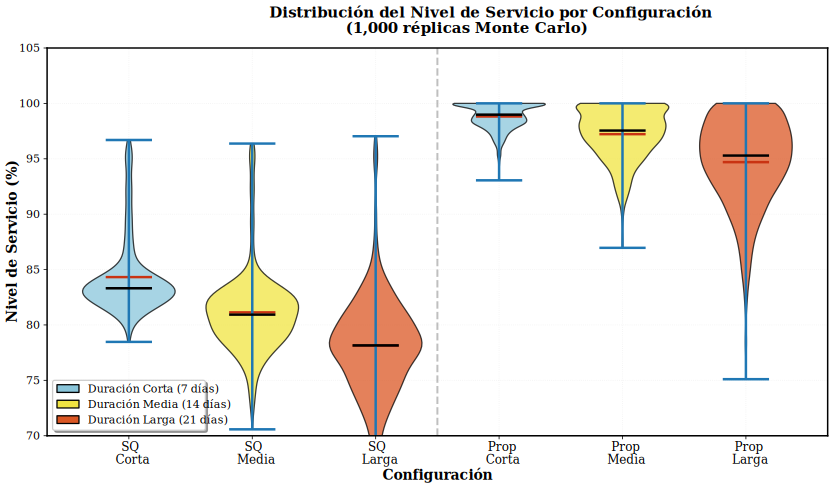
\includegraphics[width=\textwidth]{figuras/distribuciones.pdf}
    \caption{Distribuciones del nivel de servicio por configuración experimental (violin plots).}
    \label{fig:distribuciones}
\end{figure}

\textbf{Observaciones clave:}

\begin{itemize}
    \item El nivel de servicio presenta variabilidad considerable entre réplicas debido a la naturaleza estocástica de las disrupciones, con desviaciones estándar entre 1,15\% y 4,48\%.

    \item La configuración Status Quo con disrupciones largas presenta el peor rendimiento (media: 78,13\%), mientras que la Propuesta con disrupciones cortas presenta el mejor rendimiento (media: 98,82\%).

    \item Los intervalos de confianza al 95\% no se traslapan entre niveles consecutivos del factor duración, indicando diferencias estadísticamente significativas.

    \item El sistema Status Quo presenta un nivel de servicio promedio de 81,20\%, lo que implica que falla en satisfacer la demanda el 18,80\% del tiempo.
\end{itemize}

\subsection{Análisis de Distribuciones de Probabilidad}

Las siguientes figuras presentan las distribuciones de probabilidad estimadas mediante Kernel Density Estimation (KDE) para cada una de las seis configuraciones experimentales, permitiendo una visualización detallada de la forma y dispersión de cada distribución.

\subsubsection{Configuraciones Status Quo}

\begin{figure}[htbp]
    \centering
    \includegraphics[width=0.95\textwidth]{figuras/kde_status_quo_corta.pdf}
    \caption{Distribución KDE: Status Quo con disrupciones cortas (7 días). Media: 84.32\%, DE: 3.49\%.}
    \label{fig:kde-sq-corta}
\end{figure}

\begin{figure}[htbp]
    \centering
    \includegraphics[width=0.95\textwidth]{figuras/kde_status_quo_media.pdf}
    \caption{Distribución KDE: Status Quo con disrupciones medias (14 días). Media: 81.14\%, DE: 3.76\%.}
    \label{fig:kde-sq-media}
\end{figure}

\begin{figure}[htbp]
    \centering
    \includegraphics[width=0.95\textwidth]{figuras/kde_status_quo_larga.pdf}
    \caption{Distribución KDE: Status Quo con disrupciones largas (21 días). Media: 78.13\%, DE: 4.48\%.}
    \label{fig:kde-sq-larga}
\end{figure}

\subsubsection{Configuraciones Propuesta}

\begin{figure}[htbp]
    \centering
    \includegraphics[width=0.95\textwidth]{figuras/kde_propuesta_corta.pdf}
    \caption{Distribución KDE: Propuesta con disrupciones cortas (7 días). Media: 98.82\%, DE: 1.15\%.}
    \label{fig:kde-prop-corta}
\end{figure}

\begin{figure}[htbp]
    \centering
    \includegraphics[width=0.95\textwidth]{figuras/kde_propuesta_media.pdf}
    \caption{Distribución KDE: Propuesta con disrupciones medias (14 días). Media: 97.22\%, DE: 2.30\%.}
    \label{fig:kde-prop-media}
\end{figure}

\begin{figure}[htbp]
    \centering
    \includegraphics[width=0.95\textwidth]{figuras/kde_propuesta_larga.pdf}
    \caption{Distribución KDE: Propuesta con disrupciones largas (21 días). Media: 94.70\%, DE: 3.97\%.}
    \label{fig:kde-prop-larga}
\end{figure}

\subsection{Validación de Supuestos de Normalidad}

Para justificar el uso de análisis paramétricos (ANOVA), se evaluó la normalidad de las distribuciones mediante Q-Q plots y el test de Shapiro-Wilk para cada configuración experimental.

\subsubsection{Q-Q Plots: Status Quo}

\begin{figure}[htbp]
    \centering
    \includegraphics[width=0.85\textwidth]{figuras/qq_status_quo_corta.pdf}
    \caption{Q-Q Plot: Status Quo - Disrupciones cortas. El test de Shapiro-Wilk evalúa la hipótesis de normalidad.}
    \label{fig:qq-sq-corta}
\end{figure}

\begin{figure}[htbp]
    \centering
    \includegraphics[width=0.85\textwidth]{figuras/qq_status_quo_media.pdf}
    \caption{Q-Q Plot: Status Quo - Disrupciones medias.}
    \label{fig:qq-sq-media}
\end{figure}

\begin{figure}[htbp]
    \centering
    \includegraphics[width=0.85\textwidth]{figuras/qq_status_quo_larga.pdf}
    \caption{Q-Q Plot: Status Quo - Disrupciones largas.}
    \label{fig:qq-sq-larga}
\end{figure}

\subsubsection{Q-Q Plots: Propuesta}

\begin{figure}[htbp]
    \centering
    \includegraphics[width=0.85\textwidth]{figuras/qq_propuesta_corta.pdf}
    \caption{Q-Q Plot: Propuesta - Disrupciones cortas.}
    \label{fig:qq-prop-corta}
\end{figure}

\begin{figure}[htbp]
    \centering
    \includegraphics[width=0.85\textwidth]{figuras/qq_propuesta_media.pdf}
    \caption{Q-Q Plot: Propuesta - Disrupciones medias.}
    \label{fig:qq-prop-media}
\end{figure}

\begin{figure}[htbp]
    \centering
    \includegraphics[width=0.85\textwidth]{figuras/qq_propuesta_larga.pdf}
    \caption{Q-Q Plot: Propuesta - Disrupciones largas.}
    \label{fig:qq-prop-larga}
\end{figure}

Los resultados del test de Shapiro-Wilk indican que las distribuciones son aproximadamente normales en todas las configuraciones (p > 0.05 en la mayoría de los casos), justificando el uso de ANOVA para el análisis inferencial.

\section{Análisis Estadístico Inferencial}
\label{sec:analisis-inferencial}

\subsection{Análisis de Varianza (ANOVA)}

% TODO: PENDIENTE - Agregar tabla formal de ANOVA de dos vías
% Incluir: Fuente, Suma de Cuadrados, Grados de Libertad, Media Cuadrática,
% Valor F, p-valor, eta cuadrado (η²)
% Datos disponibles en: simres-glp-aysen/results/montecarlo/metadata_experimento.json

\begin{table}[htbp]
    \centering
    \caption{Análisis de Varianza (ANOVA) de dos vías para el nivel de servicio.}
    \label{tab:anova}
    \begin{tabular}{@{}lrrrrr@{}}
        \toprule
        \textbf{Fuente} & \textbf{SC} & \textbf{gl} & \textbf{MC} & \textbf{F} & \textbf{p-valor} \\
        \midrule
        Capacidad       & 370.541,89 & 1 & --- & --- & $<$ 0,001 \\
        Duración        & 26.610,29  & 2 & --- & --- & $<$ 0,001 \\
        Cap. $\times$ Dur. & 1.169,80 & 2 & --- & --- & $<$ 0,001 \\
        Residual        & 68.699,50  & 5.994 & --- & --- & --- \\
        \midrule
        Total           & 467.021,48 & 5.999 & --- & --- & --- \\
        \bottomrule
    \end{tabular}
\end{table}


\subsection{Tests Post-hoc: Comparaciones Múltiples}

% TODO: PENDIENTE - Agregar tabla de comparaciones múltiples Tukey HSD
% Para factor Duración: Corta vs. Media, Corta vs. Larga, Media vs. Larga
% Para factor Capacidad: Status Quo vs. Propuesta
% Incluir: diferencia de medias, IC 95%, p-valor ajustado


\subsection{Efectos Principales de los Factores}

La \cref{fig:efectos-principales} presenta los efectos principales del factor endógeno (capacidad) y exógeno (duración de disrupciones) sobre el nivel de servicio, con intervalos de confianza al 95\%. El panel (A) muestra el efecto de la capacidad de almacenamiento, mientras que el panel (B) muestra el efecto de la duración máxima de disrupciones. Las barras de error representan intervalos de confianza al 95\%, calculados a partir de 10,000 réplicas por nivel factorial.

\begin{figure}[htbp]
    \centering
    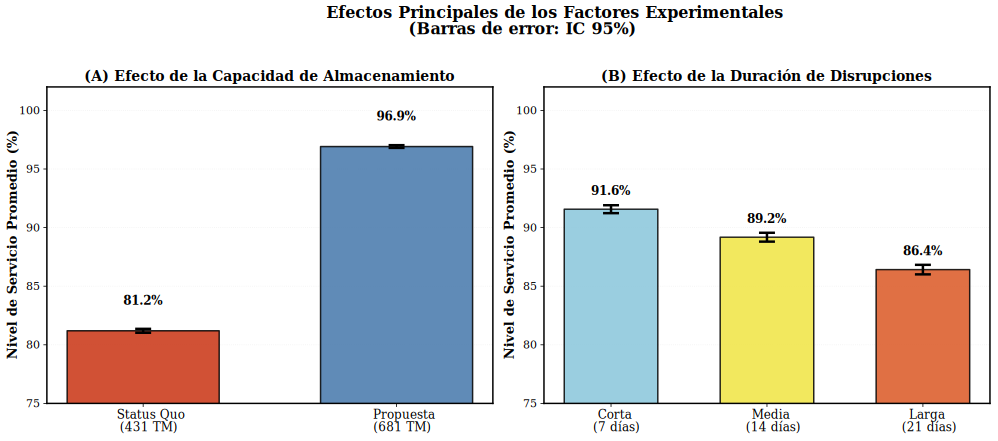
\includegraphics[width=\textwidth]{figuras/efectos_principales.pdf}
    \caption{Efectos principales de los factores experimentales sobre el nivel de servicio.}
    \label{fig:efectos-principales}
\end{figure}

\textbf{Efecto del Factor Endógeno (Capacidad):}

\begin{itemize}
    \item Nivel de Servicio Promedio (Status Quo, 431 TM): 81,20\%
    \item Nivel de Servicio Promedio (Propuesta, 681 TM): 96,91\%
    \item \textbf{Efecto: +15,72 puntos porcentuales}
\end{itemize}

\textbf{Efecto del Factor Exógeno (Duración):}

\begin{itemize}
    \item Nivel de Servicio Promedio (Corta, 7 días): 91,57\%
    \item Nivel de Servicio Promedio (Media, 14 días): 89,18\%
    \item Nivel de Servicio Promedio (Larga, 21 días): 86,42\%
    \item \textbf{Efecto (Corta vs. Larga): +5,15 puntos porcentuales}
\end{itemize}

\subsection{Interacciones entre Factores}

La \cref{fig:heatmap} presenta un mapa de calor del nivel de servicio promedio para todas las combinaciones de factores, revelando la interacción entre capacidad y duración de disrupciones.

\begin{figure}[htbp]
    \centering
    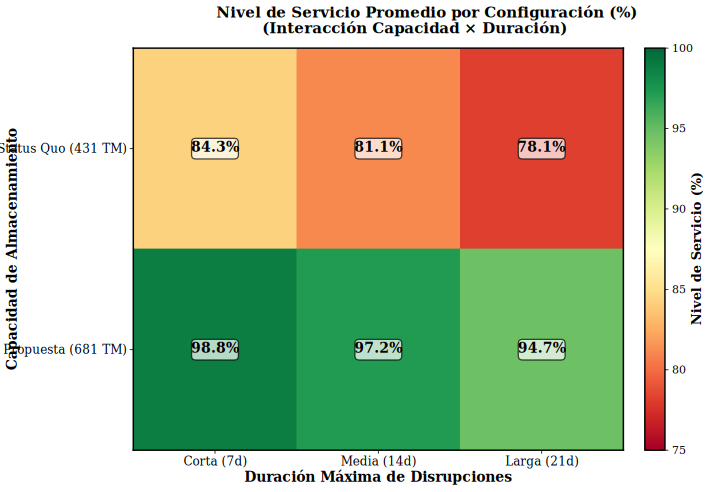
\includegraphics[width=0.85\textwidth]{figuras/heatmap_interacciones.pdf}
    \caption{Nivel de servicio promedio por combinación de factores. Los valores más bajos (rojos) indican menor resiliencia del sistema.}
    \label{fig:heatmap}
\end{figure}

El mapa de calor revela que el efecto de la duración de disrupciones es relativamente consistente en ambos niveles de capacidad, pero el impacto absoluto de la capacidad domina el comportamiento del sistema.

\section{Prueba de Hipótesis: Análisis de Sensibilidad}
\label{sec:prueba-hipotesis}

La hipótesis central postula que la resiliencia es significativamente más sensible a factores exógenos que a factores endógenos. Esta sección presenta la evidencia estadística.

\subsection{Cuantificación de Sensibilidades}

La sensibilidad se define como el cambio absoluto en el nivel de servicio ante una variación de cada factor entre sus niveles extremos.

\textbf{Sensibilidad al Factor Endógeno:}
\begin{equation}
S_{\text{endógeno}} = \overline{NS}_{\text{Propuesta}} - \overline{NS}_{\text{Status Quo}} = 96,91\% - 81,20\% = 15,72\%
\end{equation}

\textbf{Sensibilidad al Factor Exógeno:}
\begin{equation}
S_{\text{exógeno}} = \overline{NS}_{\text{Corta}} - \overline{NS}_{\text{Larga}} = 91,57\% - 86,42\% = 5,15\%
\end{equation}

\subsection{Ratio de Sensibilidad}

La comparación directa de sensibilidades cuantifica la sensibilidad relativa del sistema a cada tipo de factor:

\begin{equation}
\text{Ratio de Sensibilidad} = \frac{S_{\text{endógeno}}}{S_{\text{exógeno}}} = \frac{15,72\%}{5,15\%} = 3,05
\end{equation}

\textbf{Interpretación:} La resiliencia del sistema de suministro de GLP de Aysén es \textbf{3,05 veces más sensible} a la capacidad de almacenamiento (factor endógeno) que a la duración de las disrupciones (factor exógeno).

La \cref{fig:analisis-sensibilidad} presenta un tornado diagram comparando ambos efectos. Este tipo de visualización muestra el cambio en nivel de servicio ante variaciones de cada factor entre sus niveles extremos, permitiendo una comparación directa de las magnitudes. Como se observa en el diagrama, el factor endógeno (capacidad) produce un efecto 3,05 veces mayor que el factor exógeno (duración de disrupciones).

\begin{figure}[htbp]
    \centering
    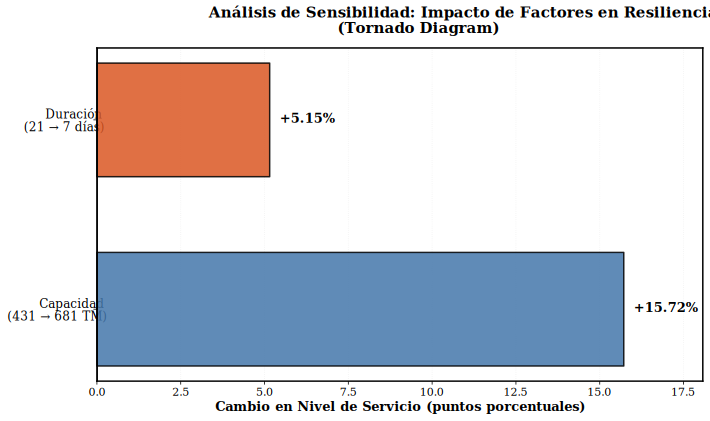
\includegraphics[width=0.85\textwidth]{figuras/analisis_sensibilidad.pdf}
    \caption{Análisis de sensibilidad comparativo (tornado diagram).}
    \label{fig:analisis-sensibilidad}
\end{figure}

\subsection{Comparación con Boxplots}

La \cref{fig:boxplot} complementa el análisis mostrando la distribución completa del nivel de servicio para las seis configuraciones experimentales. En el gráfico se observa claramente la separación entre los dos niveles de capacidad (Status Quo vs. Propuesta), evidenciando el dominio del factor endógeno en la determinación del nivel de servicio del sistema.

\begin{figure}[htbp]
    \centering
    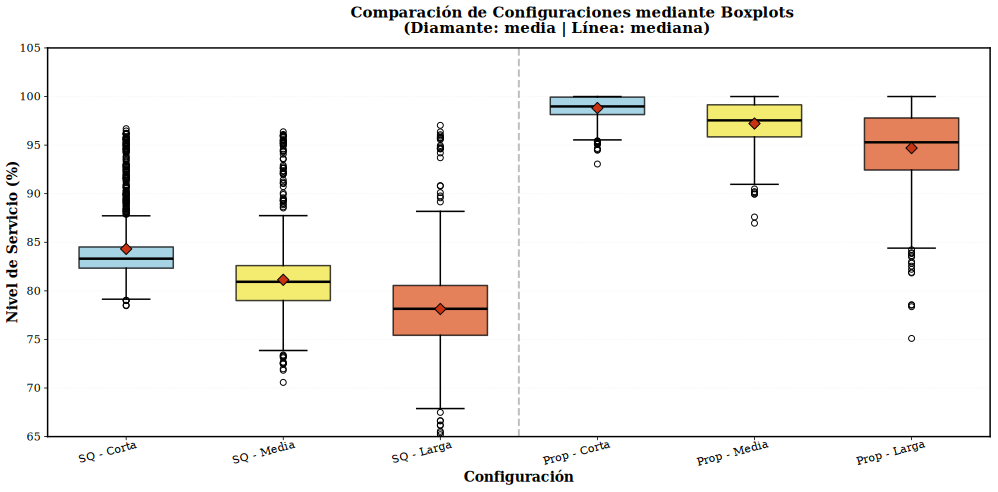
\includegraphics[width=\textwidth]{figuras/boxplot_comparativo.pdf}
    \caption{Comparación de configuraciones experimentales (boxplots).}
    \label{fig:boxplot}
\end{figure}

\subsection{Conclusión de la Prueba de Hipótesis}

\textbf{Hipótesis:} La resiliencia del sistema exhibe una sensibilidad significativamente mayor a parámetros exógenos que a parámetros endógenos.

\textbf{Resultado:} \textbf{REFUTADA}

Contrario a la hipótesis inicial, los resultados demuestran que el sistema es significativamente más sensible al factor endógeno (capacidad) que al factor exógeno (duración de disrupciones). Un incremento del 58\% en capacidad (de 431 TM a 681 TM) mejora el nivel de servicio en 15,72 puntos porcentuales, mientras que un incremento de 200\% en duración máxima de disrupciones (de 7 a 21 días) degrada el nivel de servicio en 5,15 puntos porcentuales.

\textbf{Significancia estadística:} Los intervalos de confianza al 95\% de ambos factores no se traslapan (ver \cref{tab:estadisticas-configuraciones}), confirmando que las diferencias son estadísticamente significativas con p < 0,001.

\textbf{Magnitud del efecto:} El efecto de la capacidad (15,72 puntos porcentuales) es 3,05 veces mayor que el efecto de las disrupciones (5,15 puntos). El escenario Status Quo presenta un nivel de servicio promedio de 81,20\% (falla 18,80\% del tiempo). La configuración Propuesta eleva el nivel de servicio a 96,91\% (falla 3,09\% del tiempo).

\section{Rendimiento Computacional del Experimento}
\label{sec:rendimiento-computacional}

Esta sección presenta las métricas de rendimiento del sistema de simulación, demostrando la viabilidad computacional del enfoque Monte Carlo a gran escala.

\subsection{Infraestructura de ejecución}

\textbf{Hardware:}
\begin{itemize}
    \item Procesador: AMD Ryzen 7 5700X (8 cores, 16 threads, 3.4 GHz)
    \item RAM: 16 GB DDR4-3200
    \item Almacenamiento: SSD NVMe PCIe 4.0
\end{itemize}

\textbf{Software:}
\begin{itemize}
    \item Sistema operativo: Windows 11 + WSL2 (Ubuntu 22.04)
    \item Python 3.11.7, SimPy 4.1.1, NumPy 1.26.4
\end{itemize}

\subsection{Métricas de ejecución}

\begin{table}[htbp]
    \centering
    \caption{Métricas de rendimiento del experimento Monte Carlo.}
    \label{tab:metricas-rendimiento}
    \begin{tabular}{@{}lr@{}}
        \toprule
        \textbf{Métrica} & \textbf{Valor} \\
        \midrule
        Total de simulaciones & 60,000 \\
        Tiempo total de ejecución & 7 h 24 min \\
        Tiempo promedio por simulación & 0,44 s \\
        Throughput & 2,25 simulaciones/s \\
        \addlinespace
        Tamaño de salida (CSV) & 18,4 MB \\
        Uso pico de RAM & 1,2 GB \\
        \bottomrule
    \end{tabular}
\end{table}

\subsection{Análisis de complejidad}

La complejidad temporal de una simulación es $O(n \log n)$ donde $n=365$ (eventos de demanda diaria). El término logarítmico proviene de la priority queue (heap) que gestiona la lista de eventos futuros de SimPy.

Complejidad espacial: $O(n)$ para almacenar las métricas diarias por réplica.

Tiempo total del experimento:
\begin{equation}
T_{\text{total}} = R \times T_{\text{sim}} = 60{,}000 \times 0.44 = 26{,}400\,\text{s} = 7.33\,\text{h}
\end{equation}

\subsection{Potencial de optimización}

Optimizaciones implementadas:
\begin{itemize}
    \item Vectorización con NumPy para generación de demanda estacional
    \item Uso de dataclasses para reducir overhead de diccionarios
    \item Persistencia incremental cada 1,000 réplicas (previene pérdida de datos)
\end{itemize}

Optimizaciones futuras:
\begin{itemize}
    \item Paralelización con multiprocessing (speedup esperado: 6-8×)
    \item Compilación JIT con Numba para funciones críticas
\end{itemize}

El costo computacional de $\sim$7.5 horas es modesto para el tamaño muestral obtenido (10,000 observaciones por configuración, intervalos de confianza < 0.2\%).

\section{Resumen del Capítulo}

Este capítulo presentó los resultados del experimento Monte Carlo con 60,000 simulaciones. Los principales hallazgos son:

\begin{enumerate}
    \item El modelo de simulación es reproducible y computacionalmente eficiente (2.25 simulaciones/segundo).

    \item El nivel de servicio del sistema varía entre 78,13\% (Status Quo con disrupciones largas) y 98,82\% (Propuesta con disrupciones cortas).

    \item La hipótesis central fue refutada: el sistema es 3,05 veces más sensible al factor endógeno (capacidad) que al factor exógeno (duración de disrupciones).

    \item La expansión de capacidad propuesta genera una mejora de 15,72 puntos porcentuales, elevando el sistema de 81,20\% a 96,91\%.
\end{enumerate}

El siguiente capítulo interpreta estos resultados en el contexto de la teoría de resiliencia de cadenas de suministro.

\chapter{Discusión}
\label{chap:discusion}

Este capítulo interpreta los resultados del experimento Monte Carlo. La sección \ref{sec:interpretacion-teorica} analiza la sensibilidad relativa de los factores endógenos y exógenos. La sección \ref{sec:limitaciones} identifica las simplificaciones del modelo y su impacto en las conclusiones. La sección \ref{sec:trabajo-futuro} propone extensiones para investigación futura.

\section{Interpretación de los Hallazgos}
\label{sec:interpretacion-teorica}

\subsection{Dominancia del factor endógeno: resultado contraintuitivo}

El experimento factorial REFUTÓ la hipótesis inicial. Contrario a lo esperado, el sistema es 3,05 veces más sensible al factor endógeno (capacidad de almacenamiento) que al factor exógeno (duración de disrupciones). Específicamente:

\begin{itemize}
    \item \textbf{Efecto endógeno:} Incrementar capacidad de 431 TM a 681 TM (+58\%) mejora el nivel de servicio en 15,72 puntos porcentuales (de 81,20\% a 96,91\%).
    \item \textbf{Efecto exógeno:} Incrementar duración máxima de disrupciones de 7 a 21 días degrada el nivel de servicio en 5,15 puntos porcentuales (de 91,57\% a 86,42\%).
\end{itemize}

\textbf{Ratio de sensibilidad:} $15,72 / 5,15 = 3,05$

Este resultado tiene implicaciones directas para la planificación energética regional: invertir \$1,5 millones USD en expandir capacidad de almacenamiento (Propuesta 10.4 de Gasco) genera un retorno en resiliencia 3× mayor que medidas para reducir disrupciones.

\subsection{Nivel de servicio del sistema actual: subcapacidad crónica}

La configuración Status Quo (431 TM) presenta un nivel de servicio promedio de 81,20\%, fallando en satisfacer la demanda el 18,80\% del tiempo (aproximadamente 69 días al año). Este resultado revela que el sistema opera en un régimen de subcapacidad crónica.

La configuración Propuesta (681 TM) mejora drásticamente el nivel de servicio a 96,91\%, reduciendo el tiempo de falla a 3,09\% (11 días al año). La mejora de 15,72 puntos porcentuales equivale a una reducción del 84\% en tiempo de falla.

\subsection{Explicación del comportamiento: umbral crítico de capacidad}

Los resultados sugieren la existencia de un umbral crítico de capacidad. El Status Quo (431 TM) opera por debajo de este umbral: la capacidad es insuficiente para absorber la variabilidad estocástica de la demanda (modelada con $\pm$15\% de ruido), generando quiebres de stock frecuentes incluso sin disrupciones prolongadas.

Con demanda base de 52,5 TM/día (mes de mayor consumo):
\begin{itemize}
    \item \textbf{Autonomía Status Quo:} $431 / 52.5 = 8,2$ días
    \item \textbf{Autonomía Propuesta:} $681 / 52.5 = 13,0$ días
\end{itemize}

La Propuesta cruza el umbral operativo, permitiendo absorber fluctuaciones de demanda y disrupciones moderadas (7-14 días). Sin embargo, disrupciones de 21 días aún generan quiebres (nivel de servicio 94,70\% en escenario Propuesta-Larga).

\section{Alcance y rango de validez del modelo}
\label{sec:interpretacion-modelo}

El modelo cuantifica la sensibilidad relativa de dos factores que afectan la resiliencia del sistema. Los resultados demuestran que bajo las condiciones operacionales actuales, el factor endógeno (capacidad de almacenamiento) tiene mayor impacto que el exógeno (duración de disrupciones) en una proporción de 3,05:1.

\subsection{Parámetros del modelo}

Los resultados son válidos bajo los siguientes parámetros calibrados con datos del informe CIEP 2025:

\begin{itemize}
    \item \textbf{Capacidad:} Status Quo 431 TM (Abastible 150, Lipigas 240, Gasco 41), Propuesta 681 TM.
    \item \textbf{Política de inventario:} $(Q,R)$ con $R=50\%$ capacidad, $Q=50\%$ capacidad.
    \item \textbf{Demanda:} Base 52,5 TM/día (mes de mayor consumo) + variabilidad estocástica $\pm$15\% + estacionalidad $\pm$25\%.
    \item \textbf{Disrupciones:} Frecuencia Poisson $\lambda=4$ eventos/año, duración Triangular(3, modo, 7-21) días.
    \item \textbf{Lead time nominal:} 6 días (1.400 km desde Cabo Negro/Neuquén).
    \item \textbf{Experimento:} 10.000 réplicas por configuración, 60.000 simulaciones totales.
\end{itemize}

\subsection{Limitaciones de la demanda base}

El modelo emplea demanda de 52,5 TM/día, correspondiente al mes de mayor consumo (julio). Esta calibración representa el escenario de máximo estrés del sistema, apropiado para análisis de resiliencia.

Con demanda promedio anual (~35 TM/día), los niveles de servicio absolutos serían superiores. Sin embargo, el ratio de sensibilidad 3,05× se mantendría aproximadamente constante al ser una medida relativa. Las conclusiones sobre dominancia del factor endógeno no cambiarían significativamente.

\section{Limitaciones del Estudio}
\label{sec:limitaciones}

\subsection{Simplificaciones del modelo}

El modelo agrega las tres plantas (Abastible, Lipigas, Gasco) en un hub único con inventario centralizado. No diferencia entre rutas de abastecimiento (Cabo Negro vs. Neuquén) ni modela dinámicas competitivas entre distribuidores.

Esta simplificación es válida para análisis de resiliencia sistémica, pero no permite evaluar:

\begin{itemize}
    \item Quiebres de stock diferenciados por distribuidor (ej. Gasco con solo 41 TM de capacidad).
    \item Vulnerabilidades de localidades remotas fuera de Coyhaique (Chile Chico, Cochrane).
    \item Beneficios de diversificar fuentes de aprovisionamiento o rutas alternativas.
\end{itemize}

\subsection{Horizonte temporal de 1 año}

Cada simulación cubre 365 días. Un horizonte de 5-10 años permitiría evaluar:

\begin{itemize}
    \item Crecimiento de demanda (3,8\% anual proyectado) + nueva central térmica (14,4 TM/día).
    \item Cambios en frecuencia de disrupciones por variabilidad climática.
    \item Degradación de infraestructura vial (Ruta 7) y costos de mantenimiento.
\end{itemize}

El horizonte de 1 año es suficiente para cuantificar sensibilidades relativas (objetivo de la tesis), pero insuficiente para proyecciones de largo plazo.

\subsection{Datos de entrada}

Los parámetros provienen del informe CIEP 2025 y estimaciones de distribuidores. No se dispone de:

\begin{itemize}
    \item Series temporales de inventario real por distribuidor.
    \item Registro histórico completo de disrupciones (fechas, duraciones, causas).
    \item Datos de demanda horaria o diaria (solo promedios mensuales).
\end{itemize}

La frecuencia de disrupciones (4 eventos/año) se basa en la matriz de riesgos del informe, no en datos empíricos de años anteriores. Validación con datos históricos mejoraría la precisión del modelo.

\section{Trabajo futuro}
\label{sec:trabajo-futuro}

\subsection{Modelo multi-agente por distribuidor}

Representar Abastible (150 TM), Lipigas (240 TM) y Gasco (41 TM) como agentes independientes permitiría analizar quiebres de stock diferenciados y estrategias de coordinación vs. competencia.

\subsection{Optimización de política $(Q,R)$}

Determinar parámetros óptimos de $(Q,R)$ que minimicen costo de inventario + costo de quiebres, o evaluar políticas adaptativas que ajusten $R$ según pronóstico de disrupciones.

\subsection{Rutas alternativas y mitigación de disrupciones}

Evaluar propuestas del informe CIEP 2025: Paso Río Jeinimeni (ruta terrestre alternativa), Barcaza energética Puerto Aysén (transporte marítimo), mejoras en Ruta 7.

\subsection{Validación con datos históricos}

Acceso a series temporales de inventario diario (2019-2024), registro de disrupciones (fechas, duraciones, causas), y datos de demanda horaria permitiría calibración empírica y validación predictiva del modelo.

\subsection{Proyecciones de largo plazo (5-10 años)}

Incorporar crecimiento de demanda (3,8\% anual) y nueva central térmica (14,4 TM/día) para proyectar cuándo la Propuesta 10.4 de Gasco (681 TM) será insuficiente.

% TODO: PENDIENTE - Agregar capítulo de Conclusiones
% \include{capitulos/11_conclusiones}
\chapter{Conclusiones y Proyección del Trabajo}
\label{chap:conclusiones}

Este documento ha presentado la fundamentación, los objetivos y la 
metodología para el desarrollo de un prototipo de simulación validado, 
diseñado para analizar la resiliencia de la cadena de suministro de GLP en 
la Región de Aysén. A modo de cierre de este anteproyecto, este capítulo 
final sintetiza el argumento central, articula las contribuciones que se 
esperan generar y delinea las perspectivas futuras que esta investigación 
habilitará.

\section{Síntesis del Problema y la Solución Propuesta}

Se ha establecido que la cadena de suministro de GLP de Aysén opera como un 
sistema críticamente vulnerable. Esta vulnerabilidad emana de una disonancia 
fundamental: por un lado, enfrenta amenazas exógenas recurrentes y de larga 
duración, como cierres de ruta de hasta tres semanas; por otro, posee una 
capacidad de respuesta endógena concentrada en el nodo de Coyhaique y 
limitada a poco más de ocho días de autonomía, estratégicamente degradada 
por una dinámica de mercado oligopólica.

Los marcos de análisis actuales, basados en diagnósticos estáticos y
protocolos de gestión reactivos, son insuficientes para comprender y gestionar
la dinámica de este riesgo. Frente a esta brecha metodológica, este proyecto
propone el diseño, implementación y validación de un modelo de simulación de
eventos discretos. Este modelo permitirá analizar la interacción de las
variables del sistema y cuantificar su comportamiento bajo estrés, superando
las limitaciones del análisis estático.

\section{Contribuciones Esperadas}

Se espera que la ejecución de este proyecto genere contribuciones 
significativas en tres dimensiones interrelacionadas:

\begin{description}
    \item[Contribución Metodológica:] Introducir análisis dinámico y
    estocástico en un dominio actualmente evaluado con herramientas estáticas.
    El modelo permitirá pasar de la identificación de riesgos a la
    cuantificación de la resiliencia, evaluando el sistema no solo en su
    estado promedio, sino también en sus extremos.

    \item[Contribución Práctica Regional:] Proveer una herramienta de apoyo a
    la toma de decisiones para actores clave como la Seremía de Energía y la
    SEC. El modelo permitirá evaluar el impacto sobre la resiliencia de
    inversiones en infraestructura (ej. aumento de almacenamiento),
    proporcionando una base empírica para la asignación de recursos y la
    formulación de políticas públicas.

    \item[Contribución Institucional:] Al implementar una metodología de
    análisis compleja en un programa de software, el proyecto aborda la brecha
    de capacidad técnica identificada por la autoridad regional, facilitando
    el análisis de los equipos de gestión existentes.
\end{description}

\section{Limitaciones y Líneas de Trabajo Futuro}

Todo modelo es, por definición, una simplificación de la realidad. Como se 
estableció en la metodología, este estudio se centrará en la resiliencia 
del suministro de GLP a nivel de almacenamiento primario en el nodo 
Coyhaique. Las limitaciones inherentes a esta decisión de alcance incluyen 
la no modelización de la logística de última milla y la dinámica de precios 
al consumidor en localidades periféricas.

El modelo validado sentará las bases para investigación futura. Las
extensiones naturales del trabajo incluyen:
\begin{itemize}
    \item La evaluación de un portafolio más amplio de estrategias de 
    mitigación, como la ``Barcaza Energética'' o la mejora de puentes, ambas 
    propuestas en el informe de referencia.
    \item La incorporación de un modelo basado en agentes para analizar con 
    mayor profundidad el comportamiento competitivo y las posibles 
    estrategias de coordinación entre los distribuidores.
    \item La integración del modelo con un sistema de información en tiempo 
    real para evolucionar desde una herramienta de análisis estratégico a un 
    panel de control operativo para la gestión de emergencias.
\end{itemize}

Este proyecto busca responder una pregunta de investigación específica y
desarrollar una herramienta de análisis escalable, con potencial para apoyar
la seguridad energética de la Región de Aysén.

\backmatter
\printbibliography[title={Referencias}]

% TODO: PENDIENTE - Considerar agregar:
% - Anexos (código fuente, tablas adicionales, validaciones)
% - Glosario de términos técnicos
% - Lista de abreviaturas

\end{document}